%% ===========================================================================
%%  CivicDividendOS: A Factor-Origin Fiscal Ledger and Public Automation
%%  Dividend Framework for Human--AI--Robot Economies
%%
%%  Compile:  pdflatex -> bibtex -> pdflatex -> pdflatex
%%  Requires: IEEEtran.cls, IEEEtran.bst, tikz, pgfplots, algorithmicx
%%
%%  NOTE: the class option is [journal]. To revert to the original
%%  conference format, change [journal] to [conference] below and delete
%%  the \markboth and \IEEEpeerreviewmaketitle lines.
%% ===========================================================================
\documentclass[journal]{IEEEtran}

\usepackage{amsmath,amssymb}
\let\proof\relax
\let\endproof\relax
\usepackage{amsthm}
\usepackage{cite}
\usepackage{url}
\usepackage{booktabs}
\usepackage{array}
\usepackage{microtype}
\usepackage{tikz}
\usepackage{pgfplots}
\usepackage{algorithm}
\usepackage{algpseudocode}

\usetikzlibrary{arrows.meta,positioning,calc,fit,backgrounds}
\pgfplotsset{compat=newest}

\definecolor{cdMeasure}{RGB}{222,235,247}
\definecolor{cdAttrib}{RGB}{226,240,226}
\definecolor{cdAssess}{RGB}{253,235,214}
\definecolor{cdDistrib}{RGB}{237,229,244}
\definecolor{cdGov}{RGB}{240,240,240}

\theoremstyle{plain}
\newtheorem{proposition}{Proposition}
\theoremstyle{definition}
\newtheorem{definition}{Definition}
\newtheorem{assumption}{Assumption}
\newtheorem{remark}{Remark}

\newcommand{\ACB}{\mathrm{ACB}}
\newcommand{\SAC}{\mathrm{SAC}}
\newcommand{\PAWF}{\mathrm{PAWF}}
\newcommand{\AEAP}{\mathrm{AEAP}}
\newcommand{\Rev}{\mathrm{Rev}}
\newcommand{\clip}{\operatorname{clip}}

\begin{document}

\title{CivicDividendOS: A Factor-Origin Fiscal Ledger and Public Automation Dividend Framework for Human--AI--Robot Economies}

\author{Author~Name%
\thanks{The author is with Affiliation, City, Country (e-mail: author@example.edu).}%
\thanks{Manuscript received Month DD, YYYY; revised Month DD, YYYY.}}

\markboth{Journal Name, Vol.~XX, No.~X, Month~YYYY}{Author \MakeLowercase{\textit{et al.}}: CivicDividendOS: A Factor-Origin Fiscal Ledger for Human--AI--Robot Economies}

\maketitle

\begin{abstract}
The diffusion of agentic artificial intelligence and embodied robotics is weakening the historical correspondence between human work, wages, payroll contributions, and household income. Existing proposals ask whether robots should be taxed and at what rate, or shift the fiscal burden toward capital and corporate profit; they do not resolve the prior accounting question of which factor created value when a firm or public service is jointly operated by humans, AI agents, robots, data, and conventional capital. This paper develops CivicDividendOS, a three-layer factor-origin fiscal and distribution framework. A measurement layer assigns each economically significant autonomous deployment an Autonomous Economic Activity Passport, creating an auditable economic identity---owner of record, jurisdiction, task class, resource use, and metered output---without conferring legal personality on machines. An attribution layer allocates value added across five productive factors using a Shapley-consistent estimator whose efficiency axiom guarantees budget balance and precludes double counting, and classifies each deployment as substitution, augmentation, new-task, or safety replacement. A fiscal layer applies a bounded adaptive Social Automation Contribution to the owner of record, recycles part of the proceeds through a Human Earned-Income Shield, and channels the remainder together with equity contributions into a Public Automation Wealth Fund serving citizen dividends, worker-transition insurance, human-capability investment, and public services. We state the framework's accounting identities and establish budget balance, rate boundedness and monotonicity, a Lipschitz bound on the fiscal cost of classifier misclassification, and a closed-form condition under which the fund attains a stable ratio to output. A comparative-statics result shows that the steady-state per-capita dividend decreases in the fund's payout ratio precisely when the fund return exceeds the growth rate of output. We then evaluate the framework in a heterogeneous-agent testbed against six policy baselines over 50 seeds. Two results qualify the design. The contribution base as first specified deducts machine costs in full against an inframarginal attributed value, which makes it marginally subsidise the automation it is meant to price; deducting at most half of those costs repairs this, and the corrected variant improves on the baseline in output, hours, labour share, inequality and the tax rate on work simultaneously, which no other arm achieves. Targeted transfers nonetheless remain superior for near-term poverty reduction, because a wealth fund accumulates over decades.
\end{abstract}

\begin{IEEEkeywords}
AI taxation, robot tax, automation, fiscal policy, public finance, value attribution, Shapley value, income distribution, universal basic capital, sovereign wealth fund, future of work, social dividend.
\end{IEEEkeywords}

\IEEEpeerreviewmaketitle

\section{Introduction}

\IEEEPARstart{M}{odern} tax systems were designed around economies in which human work generates wages, employers remit payroll contributions, households pay income and consumption taxes, and owners receive taxable profits from capital. Automation has always complicated this structure, but agentic AI and increasingly autonomous robots introduce a qualitatively broader challenge: software agents now execute cognitive, administrative, creative, analytical, and commercial tasks, while robots perform physical activities previously requiring human workers \cite{AcemogluRestrepo2019,BrynjolfssonMitchellRock2018,Eloundou2023}.

The economic output of a firm or municipal service may therefore arise from a joint production process involving humans, AI agents, robots, training data, cloud infrastructure, intellectual property, and conventional capital. If labour's share of production falls, governments face a structural mismatch in which the tax base remains strongly linked to wages and payroll while economic value increasingly accrues to owners of automated productive capital \cite{IMF2024Fiscal,Korinek2026}.

The policy question is not simply whether a robot should ``pay tax.'' A robot or AI agent does not possess tax residence, citizenship, consumption needs, pension rights, or legal responsibility analogous to a human worker, and current legal analysis treats AI and robots as assets, tools, services, or components of businesses rather than independent taxable persons \cite{DimitropoulouAIIncome}. The harder problem is how to attribute economic value produced through autonomous systems, and how to distribute a reasonable share of the resulting surplus without suppressing socially valuable innovation.

\subsection{Three Unresolved Gaps}

We identify three gaps that existing instruments do not jointly close. The \emph{attribution gap} is that robot counts, robot investment, imputed machine wages, and firm-level profit are all poor proxies for the economic value created by autonomous systems: one AI agent may perform the work of many humans at negligible marginal cost, another may merely augment employees, a robot may perform a hazardous task that policy should encourage, and a cloud-hosted agent may serve many jurisdictions at once. The \emph{liability gap} is that assigning machines fictional salaries and income-tax obligations is legally and administratively unworkable, because machines do not own their output and the economically relevant beneficiary is an owner, firm, platform, or operator. The \emph{distribution gap} is that current proposals typically select a single redistribution mechanism---a robot tax, higher capital taxation, universal basic income, retraining, or public ownership---whereas an AI-era economy plausibly requires several simultaneously, since displaced workers have immediate transition needs, future workers need education, households may need a non-wage income source, governments need stable revenue, and innovation still requires private returns.

\subsection{Contributions}

This paper makes the following contributions.

\begin{enumerate}
\item A \emph{factor-origin accounting layer} that allocates value added across human labour, AI-agent services, robotic services, data, and conventional capital using a Shapley-consistent estimator, together with a proof that the resulting fiscal base is budget balanced and free of double counting (Proposition~\ref{prop:balance}).
\item An \emph{Autonomous Economic Activity Passport} that creates an auditable economic identity for machine activity and binds it to a human or corporate owner of record, thereby separating machine-level economic measurement from legal tax liability.
\item A \emph{bounded adaptive Social Automation Contribution} whose rate responds to substitution, rent concentration, displacement, externalities, and base erosion, and is reduced by augmentation, training, broad-ownership, and new-task credits; we establish boundedness and monotone comparative statics (Proposition~\ref{prop:bounded}) and a Lipschitz bound on the fiscal cost of classifier error (Proposition~\ref{prop:robust}).
\item A \emph{Human Earned-Income Shield} that recycles automation revenue into reduced tax burdens on human work, with an explicit revenue-feasibility condition and a first-order behavioural correction (Proposition~\ref{prop:shield}).
\item A \emph{Public Automation Wealth Fund} converting part of automation rents into broadly owned capital, for which we derive the stability condition and closed-form steady state (Proposition~\ref{prop:fund}) and show that the steady-state per-capita dividend is decreasing in the payout ratio precisely when the fund return exceeds output growth (Proposition~\ref{prop:rg}).
\item A \emph{Deployment Nexus} apportionment rule for cross-border autonomous activity that is exhaustive by construction and deliberately excludes server location as a weighting factor (Proposition~\ref{prop:nexus}).
\item A characterisation of the \emph{marginal incidence} of the contribution base (Proposition~\ref{prop:margin}), which shows that deducting machine costs in full makes the levy marginally subsidising, and a corrected base that removes the defect.

\item A \emph{reproducible evaluation} in a heterogeneous-agent testbed against six baselines over 50 seeds, reported with paired bootstrap confidence intervals, together with governance safeguards on the use of simulation output in statutory rate setting.
\end{enumerate}

\subsection{Organization}

Section~\ref{sec:related} reviews related work and positions the framework. Section~\ref{sec:problem} formalizes the problem, states assumptions, and lists research questions. Section~\ref{sec:framework} presents the measurement and attribution layers. Section~\ref{sec:sac} develops the adaptive contribution. Section~\ref{sec:recycle} covers recycling and predistribution. Section~\ref{sec:nexus} addresses cross-border apportionment. Section~\ref{sec:waterfall} presents the distribution waterfall and annual fiscal cycle. Section~\ref{sec:twin} describes the fiscal digital twin and its governance constraints. Section~\ref{sec:example} works a numerical example end to end. Section~\ref{sec:eval} specifies the evaluation protocol. Sections~\ref{sec:discussion} and \ref{sec:limitations} discuss implications and limitations, and Section~\ref{sec:conclusion} concludes.

\section{Related Work}
\label{sec:related}

\subsection{Automation, Tasks, Wages, and Income Distribution}

A central insight in the economics of automation is that technology changes the allocation of tasks between labour and capital. Acemoglu and Restrepo show that automation produces a displacement effect by allowing capital to perform tasks previously undertaken by labour, while the creation of new tasks can reinstate labour demand \cite{AcemogluRestrepo2019}. This task-based perspective is the natural foundation for fiscal analysis because automation affects not only aggregate productivity but also who receives the associated income, an emphasis that extends the earlier routine-task literature \cite{AutorLevyMurnane2003}.

Empirical evidence indicates that the labour-market effects of robot adoption are uneven. Acemoglu and Restrepo document adverse employment and wage effects in U.S. local labour markets exposed to industrial robots \cite{AcemogluRestrepo2020}, whereas Dauth et al. find that manufacturing displacement in Germany was offset by service-sector employment, with the burden falling disproportionately on younger labour-market entrants \cite{Dauth2021}. Automation can therefore generate both gains and adjustment costs, with distributional consequences that differ across time, workers, and institutional environments.

Recent AI research broadens these concerns because AI affects non-routine cognitive tasks in addition to routine physical or clerical work \cite{FreyOsborne2017,BrynjolfssonMitchellRock2018,Eloundou2023}. The IMF emphasizes that AI may raise productivity while widening income and wealth inequality if gains accrue disproportionately to high-income workers and capital owners \cite{IMF2024AI}, and OECD evidence indicates heterogeneous effects across occupations and skill groups \cite{OECD2025Korea}.

\subsection{Robot Taxes and Optimal Taxation}

Guerreiro, Rebelo, and Teles develop a quantitative model in which falling automation costs sharply increase inequality, and find that robot taxation can be optimal during the transition while exposed workers remain in the labour force, but that the optimal tax can vanish after adjustment \cite{Guerreiro2022}. Thuemmel studies the joint taxation of robots, other capital, and labour income, showing that the optimal treatment depends on robot cost and general-equilibrium effects: subsidies may be desirable when robots are expensive, while a positive robot tax emerges as robots become cheaper and inequality rises \cite{Thuemmel2023}. Both results establish that optimal policy is dynamic rather than a permanent fixed levy.

Acemoglu et al. analyse optimal policy in a task framework and show that reducing labour taxes while combining capital-tax reductions with targeted automation taxes can improve employment outcomes relative to uniform capital taxation \cite{AcemogluOptimalPolicy}. Related work on inefficient automation finds that firms may automate too rapidly because they do not internalize transition costs borne by workers, creating an efficiency rationale for slowing automation even absent a redistributive objective \cite{InefficientAutomation}. Merola reviews taxation as a mechanism for sharing automation gains \cite{Merola2022}, and Zhang analyses automation, wage inequality, and robot taxation \cite{Zhang2019}. These contributions sit within the classical optimal-taxation tradition \cite{MirrleesOptimal1971,DiamondMirrlees1971,AtkinsonStiglitz1976}, and in particular inherit the Diamond--Mirrlees production-efficiency concern that input taxes distort factor choice unless they correct a specific externality.

The literature therefore establishes that differentiated taxation of automation may be justified under particular conditions, but a persistent implementation challenge remains: what exactly constitutes a robot, how its contribution should be measured, and how the tax can avoid discouraging beneficial capital deepening.

\subsection{Automation, the Tax Base, and AI Public Finance}

H\"{o}tte, Theodorakopoulos, and Koutroumpis examine nineteen European countries and find that the relationship between automation and tax receipts varies across technologies and diffusion phases \cite{Hotte2024}. Their results caution against assuming that automation necessarily causes a permanent decline in total revenue, while demonstrating that it can change the balance between labour, capital, and consumption tax bases. The IMF argues that fiscal policy must adapt if AI shifts income toward capital, including stronger social protection and careful consideration of capital-income taxation \cite{IMF2024Fiscal,IMF2026GlobalAI}. Korinek and co-authors develop a broader public-finance framework for advanced AI economies, analysing optimal taxation under scenarios in which capital becomes increasingly dominant \cite{Korinek2026}.

\subsection{Taxing AI Rather Than Only Robots}

Faivre and Cen survey the viability of AI taxation and distinguish multiple objectives, including correcting externalities, redistributing uneven gains and costs, and financing regulatory capacity; they discuss corporate income and rent-based taxation, consumption taxes on AI services, and excise-style instruments \cite{FaivreCen2026}. Their analysis highlights that there is unlikely to be one universal AI tax, because different harms and objectives require different bases, with measurement, incidence, international leakage, and innovation effects as the binding constraints. Legal scholarship similarly identifies substantial difficulties in treating robots or AI systems as independent taxpayers, since income-tax systems attribute income to owners, firms, or service providers rather than to the autonomous system \cite{DimitropoulouAIIncome}. This motivates separating machine-level economic measurement from legal tax liability, which is the organizing principle of the present framework.

\subsection{Transfers, Basic Capital, and Public Wealth Funds}

One response to automation is redistribution through universal basic income or targeted transfers \cite{Merola2022,VanParijs2017}, and the ILO has examined UBI proposals against social-protection standards, highlighting financing, adequacy, labour-market, and institutional questions \cite{ILOUBI}. Transfers stabilize household income but do not change the underlying ownership of productive capital, so a purely transfer-based model requires governments to tax a concentrated ownership base indefinitely. An alternative is broader asset ownership: Universal Basic Capital proposes granting citizens financial assets rather than only periodic income \cite{LeGrand2020}, and progressive sovereign wealth fund proposals argue that public ownership of capital can generate a more egalitarian distribution of investment income \cite{Corneo2022,Piketty2014}. The Alaska Permanent Fund provides a long-running example of converting resource rents into a permanent fund whose earnings support resident dividends \cite{APF}; although AI is not a natural resource, the institutional analogy is that concentrated economic rents can be partially transformed into broadly owned financial capital. Recent public-finance discussion increasingly treats equity-based mechanisms as complements to AI-era tax reform \cite{BrookingsTax2026,BrookingsFairness2026}.

\subsection{Value Attribution and Data Dividends}

Vincent et al. map design choices for data dividends and show that apparently reasonable allocation rules can generate concentrated or demographically unequal outcomes \cite{Vincent2019}, and Bax investigates Shapley- and Owen-value approaches for estimating the contribution of individual data samples \cite{Bax2019}. The cooperative-game machinery on which we draw originates with Shapley \cite{Shapley1953} and has been developed for attribution in machine learning \cite{LundbergLee2017,GhorbaniZou2019,Jia2019}. This literature is directly useful for value attribution, but data dividends address only one input into AI production and do not provide a fiscal system for joint human--AI--robot production.

\subsection{Adaptive and Agent-Based Fiscal Policy}

AI is itself being investigated as an instrument for fiscal design. TaxAgent integrates large language models with agent-based economic simulation to adapt tax policies under heterogeneous household behaviour \cite{TaxAgent2025}, the AI Economist applies two-level reinforcement learning to tax-schedule design \cite{Zheng2022AIEconomist}, and other work explores AI-supported detection of tax loopholes \cite{Fratric2025}. These systems optimize conventional tax structures; they do not establish an accounting layer identifying the factor origin of value in mixed human--agent--robot production.

\subsection{Positioning}

Table~\ref{tab:compare} positions CivicDividendOS against the principal instrument families. The distinguishing features are that the tax base is derived from attributed value added rather than asset counts or undifferentiated profit, that the statutory taxpayer is always the owner of record, that the rate is conditioned on the measured substitution--augmentation mode, and that redistribution and predistribution operate jointly rather than as alternatives.

\begin{table*}[!t]
\centering
\caption{Positioning of CivicDividendOS relative to principal fiscal instrument families for automation. ``Attribution granularity'' denotes the finest unit at which value creation is resolved.}
\label{tab:compare}
\scriptsize
\begin{tabular}{@{}l l l c c c c@{}}
\toprule
\textbf{Instrument} & \textbf{Tax base} & \textbf{Attribution} & \textbf{Statutory} & \textbf{Sub./aug.} & \textbf{Pre-} & \textbf{Cross-border} \\
 & & \textbf{granularity} & \textbf{payer} & \textbf{sensitive} & \textbf{distribution} & \textbf{rule} \\
\midrule
Fixed robot tax & Robot count / capital & Asset unit & Firm & No & No & Asset location \\
Capital-income tax increase & Capital income & Firm & Firm & No & No & Residence/source \\
Corporate rent tax & Above-normal profit & Firm & Firm & No & No & Treaty-based \\
UBI via general taxation & Aggregate revenue & None & Households & No & No & Domestic only \\
Automation tax plus retraining & Automation capital & Asset unit & Firm & Partial & No & Asset location \\
Public wealth fund only & Equity stakes & None & n/a & No & Yes & Ownership \\
Data dividend & Data contribution & Data record & Platform & No & Partial & Platform residence \\
\textbf{CivicDividendOS} & \textbf{Attributed automation VA} & \textbf{Production episode} & \textbf{Owner of record} & \textbf{Yes} & \textbf{Yes} & \textbf{Deployment nexus} \\
\bottomrule
\end{tabular}
\end{table*}

\section{Problem Formulation}
\label{sec:problem}

\subsection{Setting and Notation}

Let economic output $Y$ be jointly produced by human labour $H$, AI-agent services $A$, robotic services $R$, data $D$, and conventional capital $K$, so that $Y=F(H,A,R,D,K)$. Under a traditional fiscal system, a substantial share of public revenue is generated from

\begin{equation}
\label{eq:trad}
\mathrm{Tax}^{\mathrm{trad}} = \tau_L W_H + \tau_K \Pi + \tau_C C,
\end{equation}

where $W_H$ is human wage income, $\Pi$ taxable capital or corporate income, and $C$ consumption. As autonomous factors replace or augment human tasks, the wage share may decline while output is constant or rising,

\begin{equation}
\label{eq:shift}
\frac{W_H}{Y}\downarrow, \qquad \frac{Y_A+Y_R}{Y}\uparrow,
\end{equation}

so that if ownership of $A$ and $R$ is concentrated, household purchasing power, payroll-financed social protection, and government revenue can all weaken even as aggregate productivity rises. Table~\ref{tab:notation} summarizes the notation used throughout.

\begin{table}[!t]
\centering
\caption{Principal notation.}
\label{tab:notation}
\footnotesize
\begin{tabular}{@{}l l@{}}
\toprule
\textbf{Symbol} & \textbf{Meaning} \\
\midrule
$\mathcal{F}$ & Factor set $\{H,A,R,D,K\}$, $n=|\mathcal{F}|=5$ \\
$p$, $\mathcal{P}_i$ & Production episode; episodes of entity $i$ \\
$V_p$ & Value added of episode $p$ \\
$v_p(S)$ & Coalition value of factor subset $S\subseteq\mathcal{F}$ \\
$\psi_{p,f}$ & Shapley value of factor $f$ in episode $p$ \\
$\phi_{p,f}$ & Normalized attribution share, $\psi_{p,f}/V_p$ \\
$Z_p$ & Automation mode of episode $p$ \\
$S_i$ & Substitution intensity index of entity $i$ \\
$A^{\mathrm{aug}}_i$ & Augmentation benefit index \\
$\ACB_i$ & Automation Contribution Base \\
$r_i$ & Social Automation Contribution rate \\
$r_0$ & Base rate; $r_{\min},r_{\max}$ rate floor and ceiling \\
$\SAC_i$ & Social Automation Contribution liability \\
$\kappa$ & Share of $\SAC$ revenue recycled to the shield \\
$\omega$ & Share of $\SAC$ revenue paid into the fund \\
$F_t$ & Fund value at $t$; $f_t=F_t/Y_t$ \\
$r^{f}$ & Real fund return; $g$ real output growth \\
$\rho$ & Fund payout ratio (share of gross return) \\
$s$ & Fund inflow as a share of output \\
$N_t$ & Eligible resident population \\
$\Theta$ & Policy parameter vector \\
\bottomrule
\end{tabular}
\end{table}

\subsection{Assumptions}

The framework rests on the following assumptions, each of which is revisited in Section~\ref{sec:limitations}.

\begin{assumption}[Registrability]
\label{as:reg}
Every economically significant autonomous deployment can be registered, and its outputs metered, at the level of a production episode. Deployments below a de minimis threshold are exempt.
\end{assumption}

\begin{assumption}[Observable value added]
\label{as:va}
Episode-level value added $V_p$ is observable from accounting records, and a coalition value function $v_p:2^{\mathcal{F}}\to\mathbb{R}_{\ge 0}$ with $v_p(\emptyset)=0$ and $v_p(\mathcal{F})=V_p$ can be estimated.
\end{assumption}

\begin{assumption}[Monotone production]
\label{as:mono}
$v_p$ is monotone, i.e. $v_p(S)\le v_p(S\cup\{f\})$ for all $S\subseteq\mathcal{F}$ and $f\notin S$: adding a factor never reduces attainable value.
\end{assumption}

\begin{assumption}[Owner of record]
\label{as:owner}
Every registered deployment has a unique legally responsible owner, operator, or beneficiary. No legal personality is conferred on machines.
\end{assumption}

\begin{assumption}[Bounded classification error]
\label{as:class}
The substitution--augmentation classifier misclassifies with probability at most $\varepsilon$, and index inputs are normalized to $[0,1]$.
\end{assumption}

\begin{assumption}[Policy horizon]
\label{as:horizon}
Over the rate-adjustment horizon, firms are price takers in factor markets and the fund's real return $r^{f}$ and output growth $g$ are constant. This assumption is used only for the steady-state results of Section~\ref{sec:recycle}.
\end{assumption}

\subsection{Research Problem and Questions}

The fundamental research problem is how a tax-and-distribution system can identify the economic value created by humans, AI agents, robots, data, and conventional capital; assign legal fiscal responsibility to the appropriate human or corporate beneficiaries; and distribute part of the automation-generated surplus in a way that preserves innovation, public revenue, household income, workforce transition, and broad participation in future capital returns. The problem is harder when AI agents are cloud-hosted, operate across borders, change tasks rapidly, and act primarily as complements rather than substitutes.

This decomposes into eight research questions. \textbf{RQ1}: can task-level factor-origin accounting estimate attributable value more accurately than robot counts, imputed robot wages, or capital expenditure? \textbf{RQ2}: can a substitution--augmentation classifier distinguish automation that displaces taxable labour from automation that complements workers? \textbf{RQ3}: does a dynamic Social Automation Contribution preserve government revenue with less distortion to innovation than a fixed robot tax? \textbf{RQ4}: can combining automation contributions with a Human Earned-Income Shield improve employment and after-tax wage outcomes relative to raising labour or consumption taxes? \textbf{RQ5}: does a Public Automation Wealth Fund create a more durable and equitable distribution of AI-era wealth than transfers financed entirely from annual revenue? \textbf{RQ6}: what allocation among citizen dividends, worker transition, human-capability investment, and public services maximizes long-run social welfare? \textbf{RQ7}: how should cross-border AI-agent activity be apportioned when ownership, compute, users, and deployment occur in different jurisdictions? \textbf{RQ8}: how robust is the framework to avoidance, misclassification, strategic task decomposition, offshoring, and rapid capability change?

\section{The CivicDividendOS Framework}
\label{sec:framework}

CivicDividendOS is organized into a measurement layer, an attribution layer, and a fiscal layer, with a governance and simulation loop closing over the policy vector. Fig.~\ref{fig:arch} shows the architecture, and Table~\ref{tab:components} maps each component to the gap it addresses and the observable it requires.

\begin{figure*}[!t]
\centering
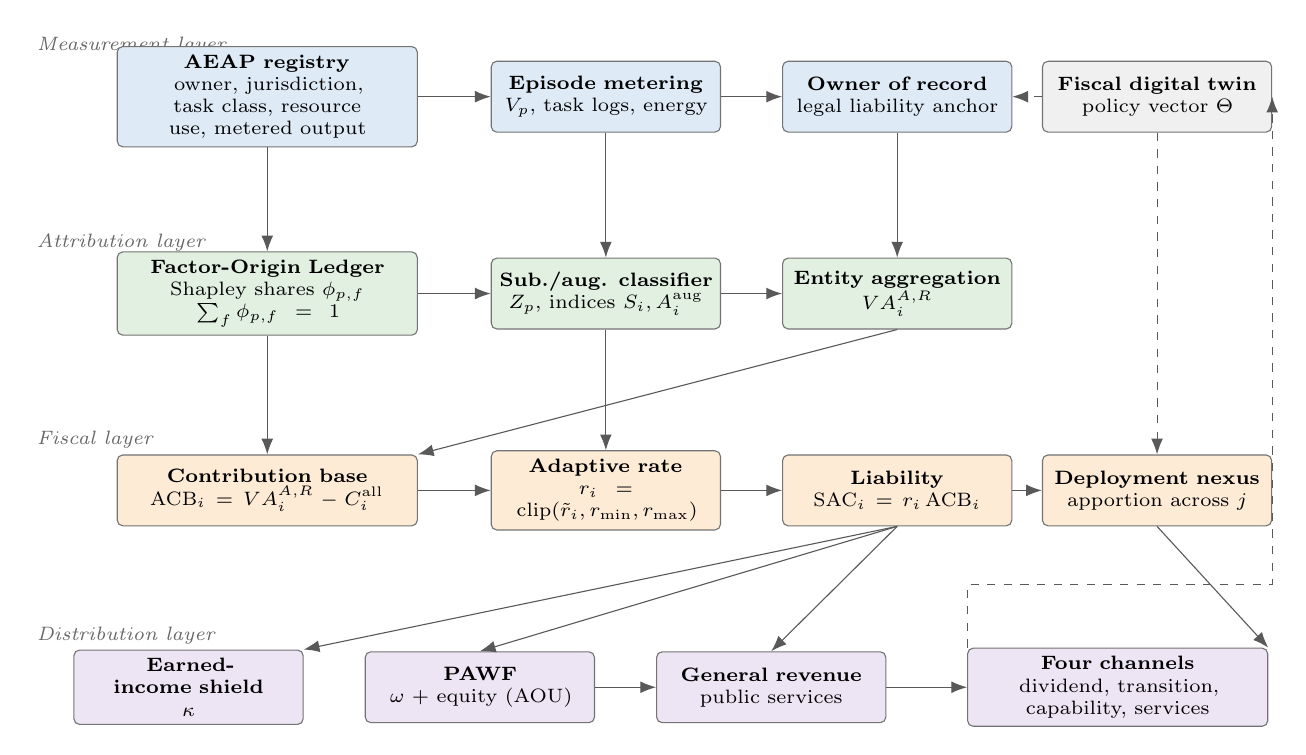
\begin{tikzpicture}[
  font=\scriptsize,
  box/.style={rounded corners=2pt, draw=black!55, minimum height=9mm, align=center, inner sep=3pt, text width=27mm},
  wide/.style={box, text width=36mm},
  arr/.style={-{Latex[length=2mm]}, draw=black!65},
  lbl/.style={font=\scriptsize\itshape, text=black!60}
]

% Band labels
\node[lbl, anchor=west] at (-0.45,0.95) {Measurement layer};
\node[lbl, anchor=west] at (-0.45,-1.55) {Attribution layer};
\node[lbl, anchor=west] at (-0.45,-4.05) {Fiscal layer};
\node[lbl, anchor=west] at (-0.45,-6.55) {Distribution layer};

% Measurement
\node[wide, fill=cdMeasure] (aeap) at (2.6,0.3) {\textbf{AEAP registry}\\owner, jurisdiction, task class, resource use, metered output};
\node[box, fill=cdMeasure] (meter) at (6.9,0.3) {\textbf{Episode metering}\\$V_p$, task logs, energy};
\node[box, fill=cdMeasure] (owner) at (10.6,0.3) {\textbf{Owner of record}\\legal liability anchor};
\node[box, fill=cdGov] (twin) at (13.9,0.3) {\textbf{Fiscal digital twin}\\policy vector $\Theta$};

% Attribution
\node[wide, fill=cdAttrib] (ledger) at (2.6,-2.2) {\textbf{Factor-Origin Ledger}\\Shapley shares $\phi_{p,f}$\\$\sum_f \phi_{p,f}=1$};
\node[box, fill=cdAttrib] (clf) at (6.9,-2.2) {\textbf{Sub./aug. classifier}\\$Z_p$, indices $S_i, A^{\mathrm{aug}}_i$};
\node[box, fill=cdAttrib] (agg) at (10.6,-2.2) {\textbf{Entity aggregation}\\$VA^{A,R}_i$};

% Fiscal
\node[wide, fill=cdAssess] (acb) at (2.6,-4.7) {\textbf{Contribution base}\\$\ACB_i = VA^{A,R}_i - C^{\mathrm{all}}_i$};
\node[box, fill=cdAssess] (rate) at (6.9,-4.7) {\textbf{Adaptive rate}\\$r_i=\clip(\tilde r_i, r_{\min}, r_{\max})$};
\node[box, fill=cdAssess] (liab) at (10.6,-4.7) {\textbf{Liability}\\$\SAC_i = r_i\,\ACB_i$};
\node[box, fill=cdAssess] (nex) at (13.9,-4.7) {\textbf{Deployment nexus}\\apportion across $j$};

% Distribution
\node[box, fill=cdDistrib] (shield) at (1.6,-7.2) {\textbf{Earned-income shield}\\$\kappa$};
\node[box, fill=cdDistrib] (fund) at (5.3,-7.2) {\textbf{PAWF}\\$\omega$ + equity (AOU)};
\node[box, fill=cdDistrib] (gen) at (9.0,-7.2) {\textbf{General revenue}\\public services};
\node[wide, fill=cdDistrib] (chan) at (13.4,-7.2) {\textbf{Four channels}\\dividend, transition, capability, services};

% Arrows
\draw[arr] (aeap) -- (meter);
\draw[arr] (meter) -- (owner);
\draw[arr] (aeap.south) -- (ledger.north);
\draw[arr] (meter.south) -- (clf.north);
\draw[arr] (ledger) -- (clf);
\draw[arr] (clf) -- (agg);
\draw[arr] (owner.south) -- (agg.north);
\draw[arr] (agg.south) -- (acb.north east);
\draw[arr] (ledger.south) -- (acb.north);
\draw[arr] (acb) -- (rate);
\draw[arr] (clf.south) -- (rate.north);
\draw[arr] (rate) -- (liab);
\draw[arr] (liab) -- (nex);
\draw[arr] (liab.south) -- (shield.north east);
\draw[arr] (liab.south) -- (fund.north);
\draw[arr] (liab.south) -- (gen.north);
\draw[arr] (fund) -- (gen);
\draw[arr] (gen) -- (chan);
\draw[arr] (nex.south) -- (chan.north east);

% Governance feedback loop
\draw[arr, dashed] (twin.south) -- (nex.north);
\draw[arr, dashed] (twin.west) -- (owner.east);
\draw[arr, dashed] (chan.north west) -- ++(0,0.8) -| (twin.east);

\end{tikzpicture}
\caption{CivicDividendOS architecture. Solid arrows carry measured or assessed quantities; dashed arrows carry policy parameters and simulation feedback. The owner of record is the sole statutory taxpayer; no fiscal obligation attaches to a machine. The digital twin proposes but does not autonomously set the policy vector $\Theta$ (Section~\ref{sec:twin}).}
\label{fig:arch}
\end{figure*}

\begin{table*}[!t]
\centering
\caption{Framework components, the gap each addresses, and the observable each requires.}
\label{tab:components}
\scriptsize
\begin{tabular}{@{}l l l l@{}}
\toprule
\textbf{Component} & \textbf{Gap addressed} & \textbf{Mechanism} & \textbf{Required observable} \\
\midrule
Autonomous Economic Activity Passport & Liability & Registry binding activity to owner of record & Registration, jurisdiction, task class, resource use \\
Factor-Origin Ledger & Attribution & Shapley allocation over five factors & Episode value added, coalition counterfactuals \\
Substitution--Augmentation Classifier & Attribution & Mode assignment $Z_p$ and index construction & Employment, hours, wage and task-level panels \\
Automation Contribution Base & Attribution & Attributed value added net of allowable cost & Verified compute, energy, depreciation costs \\
Social Automation Contribution & Distribution & Bounded adaptive rate on the base & Substitution, rent, displacement, credit indices \\
Human Earned-Income Shield & Distribution & Recycling to labour-income tax relief & Payroll base, labour supply elasticity \\
Public Automation Wealth Fund & Distribution & Fund accumulation and payout rule & Fund return, inflow share, population \\
Automation Ownership Units & Distribution & Equity contribution against public support & Subsidy, compute, data, procurement receipts \\
Deployment Nexus & Attribution & Multi-factor jurisdictional apportionment & Usage, revenue, users, physical operations \\
Fiscal Digital Twin & Distribution & Ex ante screening of policy vectors & Calibrated heterogeneous-agent model \\
\bottomrule
\end{tabular}
\end{table*}

\subsection{Measurement Layer: Autonomous Economic Activity Passport}

Every economically significant autonomous deployment $j$ is assigned an Autonomous Economic Activity Passport,

\begin{equation}
\label{eq:aeap}
\AEAP_j = \{\mathrm{ID}_j, O_j, J_j, T_j, E_j, Q_j, X_j, M_j\},
\end{equation}

where $O_j$ is the legally responsible owner or operator, $J_j$ the deployment jurisdiction, $T_j$ the task category, $E_j$ energy and resource consumption, $Q_j$ metered output, $X_j$ the risk classification, and $M_j$ the model or robot class. The record \eqref{eq:aeap} is not legal personhood; it is a fiscal measurement record that allows economic activity generated by an AI agent or robot to be audited without treating the system as a taxpayer. This construction is what operationalizes the separation of measurement from liability identified as necessary in \cite{DimitropoulouAIIncome}.

\subsection{Attribution Layer: Factor-Origin Ledger}

For each production episode $p$, the ledger estimates the causal contribution of the five factors. Let $v_p(S)$ denote the value attainable by coalition $S\subseteq\mathcal{F}$ under Assumption~\ref{as:va}. The attribution to factor $f$ is the Shapley value \cite{Shapley1953}

\begin{equation}
\label{eq:shapley}
\psi_{p,f} = \!\!\sum_{S\subseteq\mathcal{F}\setminus\{f\}}\!\! \frac{|S|!\,(n-|S|-1)!}{n!}\bigl[v_p(S\cup\{f\}) - v_p(S)\bigr],
\end{equation}

with normalized shares $\phi_{p,f} = \psi_{p,f}/V_p$ for $V_p>0$ and attributed value $V_{p,f} = \phi_{p,f}V_p$. Coalition values may be estimated through controlled counterfactuals, production-function estimation, matched historical baselines, or digital-twin simulation, following the estimation strategies developed for attribution in machine learning \cite{LundbergLee2017,GhorbaniZou2019,Jia2019}.

\begin{proposition}[Budget balance and no double counting]
\label{prop:balance}
Under Assumptions~\ref{as:va} and \ref{as:mono}, the attribution defined by \eqref{eq:shapley} satisfies $\sum_{f\in\mathcal{F}} V_{p,f} = V_p$ and $V_{p,f}\ge 0$ for every $f$. Consequently the aggregate automation base satisfies $VA^{A,R}_i \le \sum_{p\in\mathcal{P}_i} V_p$, so no unit of value added can be assessed more than once.
\end{proposition}

\begin{proof}
The Shapley value satisfies the efficiency axiom, $\sum_{f}\psi_{p,f} = v_p(\mathcal{F}) - v_p(\emptyset) = V_p$, which gives $\sum_f \phi_{p,f}=1$ and hence the first identity. Under Assumption~\ref{as:mono} every marginal contribution $v_p(S\cup\{f\})-v_p(S)$ is non-negative, and $\psi_{p,f}$ is a convex combination of such terms, so $\psi_{p,f}\ge 0$. Summing the non-negative terms $V_{p,A}+V_{p,R}\le V_p$ over $p\in\mathcal{P}_i$ yields the bound.
\end{proof}

\begin{remark}[Computational cost]
With $n=5$ factors, exact evaluation of \eqref{eq:shapley} requires only $2^{n}-1=31$ coalition values per episode, so no sampling approximation is needed at the factor level. Approximation is required only for the second-stage allocation within a factor when many distinct agents or robots must be separated, where standard Shapley samplers apply \cite{Jia2019}.
\end{remark}

This is the central departure from conventional robot taxation: the system taxes neither the physical count of robots nor a fictional machine wage, but the estimated economic origin of value.

\subsection{Substitution--Augmentation Classification}

Automation that replaces a worker and automation that makes a worker more productive should not receive identical fiscal treatment. Each episode is assigned a mode

\begin{equation}
\label{eq:mode}
\begin{split}
Z_p \in \{ &\textsc{Substitution},\ \textsc{Augmentation},\\
&\textsc{NewTask},\ \textsc{SafetyReplacement}\},
\end{split}
\end{equation}

with a substitution score $S_p = \Pr(\Delta H_p < 0 \mid A_p, R_p, \mathbf{X}_p)$ estimated from employment, hours, and task panels, and a complementary augmentation score measuring gains to human productivity or wages. Entity-level indices $S_i$ and $A^{\mathrm{aug}}_i$ are value-weighted averages of episode scores taken under the mode assignment \eqref{eq:mode}. This classification enters the rate directly, and its error properties are analysed in Proposition~\ref{prop:robust}.

\section{Adaptive Social Automation Contribution}
\label{sec:sac}

\subsection{Contribution Base and Statutory Taxpayer}

The Automation Contribution Base of entity $i$ is

\begin{equation}
\label{eq:acb}
\ACB_i = VA^{A,R}_i - C^{\mathrm{all}}_i, \qquad VA^{A,R}_i = \!\!\sum_{p\in\mathcal{P}_i}\!\! (V_{p,A}+V_{p,R}),
\end{equation}

where $C^{\mathrm{all}}_i$ comprises verified operating, compute, energy, depreciation, and acquisition costs admitted by policy. By Assumption~\ref{as:owner} the statutory taxpayer is $\mathrm{Owner}(\AEAP_i)$, never the AI agent or robot.

\subsection{Marginal Incidence of the Contribution Base}

The base \eqref{eq:acb} deducts the full cost of machine services from an attributed value that is inframarginal, and these two quantities do not have the same derivative. This has a consequence that is easy to miss and that determines whether the instrument discourages automation at all.

\begin{proposition}[Marginal incidence of the contribution base]
\label{prop:margin}
Let attribution be the Shapley value over $\{L,M\}$ of the production game with $v(\{L,M\})=Y(L,M)$, and let the firm be a price taker choosing $M$ so that $\partial Y/\partial M = p_M$. For the base $\ACB = \psi_M - \varphi\,p_M M$ with deduction share $\varphi\in[0,1]$,
\begin{equation}
\label{eq:margin}
\frac{\partial \ACB}{\partial M} = \tfrac{1}{2}\frac{\partial v(\{M\})}{\partial M} + \left(\tfrac{1}{2}-\varphi\right)p_M .
\end{equation}
Under full deduction $\varphi = 1$ this equals $\tfrac{1}{2}[\partial v(\{M\})/\partial M - p_M]$, which is negative whenever the machine's stand-alone marginal product falls below its price, so the contribution is marginally \emph{subsidising} rather than corrective. Any $\varphi \le 1/2$ restores $\partial \ACB/\partial M \ge 0$.
\end{proposition}

\begin{proof}
Since $\psi_M = \tfrac{1}{2}v(\{M\}) + \tfrac{1}{2}[v(\{L,M\}) - v(\{L\})]$ and $v(\{L\})$ does not depend on $M$, differentiating gives $\partial\psi_M/\partial M = \tfrac{1}{2}\partial v(\{M\})/\partial M + \tfrac{1}{2}\partial Y/\partial M$. Substituting the first-order condition $\partial Y/\partial M = p_M$ and subtracting $\varphi p_M$ yields \eqref{eq:margin}. Setting $\varphi = 1$ and $\varphi = 1/2$ gives the two stated cases.
\end{proof}

Proposition~\ref{prop:margin} is a design warning rather than a curiosity. The Shapley term $\psi_M$ credits the machine factor with half of the complementarity surplus it shares with labour, which is inframarginal, whereas the cost deduction $p_M M$ scales one-for-one with the marginal decision. Deducting costs in full therefore makes an additional machine reduce the taxable base, and a levy on that base lowers the effective machine price. The condition under which this bites is structural rather than empirical, and it is worth stating precisely. Under the CES-with-span-of-control technology of Section~\ref{sec:model} the ratio of the stand-alone to the joint marginal product is exactly $s_M^{\gamma/\rho-1}$ with $s_M\in(0,1)$ and $\rho = 1-1/\sigma$, so $\partial v(\{M\})/\partial M < p_M$ holds \emph{identically} whenever $\gamma > 1-1/\sigma$. At the calibration of Section~\ref{sec:model} ($\gamma=0.85$, $\sigma=1.5$) the inequality therefore cannot fail, and its universal incidence across firms and quarters is a property of the calibration rather than evidence about the world. We report it as such. The implied effective wedge at that calibration is between $-3.3\%$ and $-4.1\%$ of the machine price. We therefore evaluate both the base exactly as specified in \eqref{eq:acb} and a corrected base with $\varphi = 1/2$, and recommend the latter.

\subsection{Rate Function}

Let the raw rate score be

\begin{align}
\label{eq:rawrate}
\tilde r_i = r_0 &+ \alpha S_i + \beta C^{\mathrm{rent}}_i + \gamma E^{\mathrm{disp}}_i + \delta X^{\mathrm{ext}}_i + \eta R^{\mathrm{rev}}_i \nonumber\\
&- \theta A^{\mathrm{aug}}_i - \lambda T^{\mathrm{train}}_i - \mu B^{\mathrm{broad}}_i - \nu N^{\mathrm{new}}_i,
\end{align}

with all indices normalized to $[0,1]$ and all weights non-negative, where $S_i$ is labour substitution intensity, $C^{\mathrm{rent}}_i$ an economic-rent and concentration score, $E^{\mathrm{disp}}_i$ measured worker-displacement burden, $X^{\mathrm{ext}}_i$ environmental or social externalities, $R^{\mathrm{rev}}_i$ erosion of the payroll and social-contribution base in the sense of \eqref{eq:shift}, $A^{\mathrm{aug}}_i$ human augmentation benefit, $T^{\mathrm{train}}_i$ verified worker training and transition investment, $B^{\mathrm{broad}}_i$ a broad-ownership and benefit score, and $N^{\mathrm{new}}_i$ creation of new human tasks. The applied rate and liability are

\begin{equation}
\label{eq:rate}
r_i = \clip(\tilde r_i, r_{\min}, r_{\max}), \qquad \SAC_i = r_i \cdot \ACB_i .
\end{equation}

A differentiable alternative, $r_i = r_{\min} + (r_{\max}-r_{\min})\,\sigma(\tilde r_i)$ with $\sigma$ logistic, may be preferred when the policy vector is tuned by gradient-based search; all results below hold for either map, since both are non-decreasing and Lipschitz with constant at most one after scaling.

\begin{proposition}[Boundedness and monotone comparative statics]
\label{prop:bounded}
For any index vector, $r_i\in[r_{\min},r_{\max}]$ and hence the effective burden on attributed automation value added never exceeds $r_{\max}$. Moreover $r_i$ is non-decreasing in $S_i$, $C^{\mathrm{rent}}_i$, $E^{\mathrm{disp}}_i$, $X^{\mathrm{ext}}_i$ and $R^{\mathrm{rev}}_i$, and non-increasing in $A^{\mathrm{aug}}_i$, $T^{\mathrm{train}}_i$, $B^{\mathrm{broad}}_i$ and $N^{\mathrm{new}}_i$; the inequalities are strict wherever $\tilde r_i\in(r_{\min},r_{\max})$.
\end{proposition}

\begin{proof}
$\clip(\cdot,r_{\min},r_{\max})$ maps $\mathbb{R}$ onto $[r_{\min},r_{\max}]$ and is non-decreasing, and $\tilde r_i$ in \eqref{eq:rawrate} is affine with non-negative coefficients on the first group and non-positive coefficients on the second. A non-decreasing map composed with an affine function preserves the sign of each partial derivative, and on the open interval where the clip is inactive the composition is the identity, giving strictness. Since $\SAC_i = r_i \ACB_i$ and $\ACB_i \le VA^{A,R}_i$, the burden ratio $\SAC_i/VA^{A,R}_i \le r_{\max}$.
\end{proof}

Proposition~\ref{prop:bounded} supplies an investment-relevant guarantee: whatever the index realizations, the marginal fiscal burden on automation value added is capped at $r_{\max}$, which can be published ex ante. A complementary design condition ensures that purely complementary automation is untaxed at the floor: if $\theta \ge r_0 + \beta C^{\mathrm{rent}}_i + \eta R^{\mathrm{rev}}_i - r_{\min}$ whenever $S_i = 0$ and $A^{\mathrm{aug}}_i = 1$, then augmentation-only deployments face $r_i = r_{\min}$.

Fig.~\ref{fig:rate} plots the applied rate against substitution intensity for three augmentation levels under the calibration of Section~\ref{sec:example}, illustrating both the monotonicity of Proposition~\ref{prop:bounded} and the activation of the floor at high augmentation.

\begin{figure}[!t]
\centering
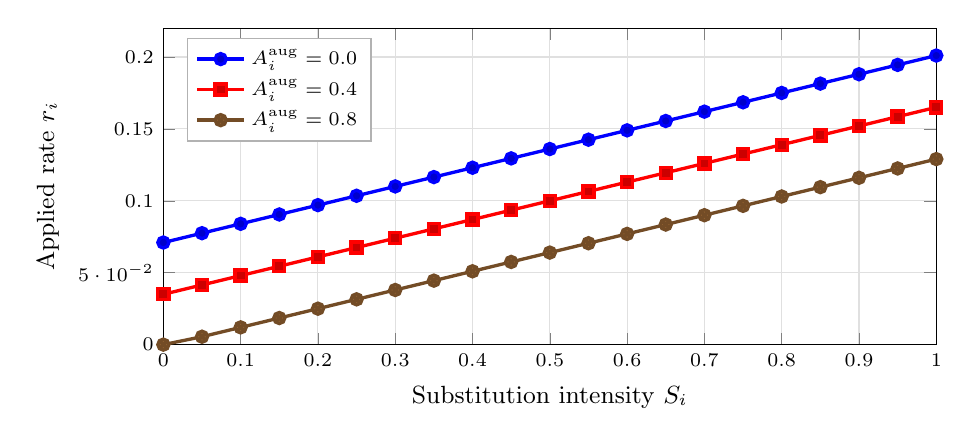
\begin{tikzpicture}
\begin{axis}[
  width=0.94\columnwidth, height=5.6cm,
  xlabel={Substitution intensity $S_i$},
  ylabel={Applied rate $r_i$},
  xmin=0, xmax=1, ymin=0, ymax=0.22,
  grid=major, grid style={black!12},
  legend pos=north west, legend cell align=left,
  legend style={font=\scriptsize, draw=black!30},
  label style={font=\small}, tick label style={font=\scriptsize},
  every axis plot/.append style={very thick, mark=none}
]
\addplot coordinates {(0.000,0.07100) (0.050,0.07750) (0.100,0.08400) (0.150,0.09050) (0.200,0.09700) (0.250,0.10350) (0.300,0.11000) (0.350,0.11650) (0.400,0.12300) (0.450,0.12950) (0.500,0.13600) (0.550,0.14250) (0.600,0.14900) (0.650,0.15550) (0.700,0.16200) (0.750,0.16850) (0.800,0.17500) (0.850,0.18150) (0.900,0.18800) (0.950,0.19450) (1.000,0.20100)};
\addlegendentry{$A^{\mathrm{aug}}_i=0.0$}
\addplot coordinates {(0.000,0.03500) (0.050,0.04150) (0.100,0.04800) (0.150,0.05450) (0.200,0.06100) (0.250,0.06750) (0.300,0.07400) (0.350,0.08050) (0.400,0.08700) (0.450,0.09350) (0.500,0.10000) (0.550,0.10650) (0.600,0.11300) (0.650,0.11950) (0.700,0.12600) (0.750,0.13250) (0.800,0.13900) (0.850,0.14550) (0.900,0.15200) (0.950,0.15850) (1.000,0.16500)};
\addlegendentry{$A^{\mathrm{aug}}_i=0.4$}
\addplot coordinates {(0.000,0.00000) (0.050,0.00550) (0.100,0.01200) (0.150,0.01850) (0.200,0.02500) (0.250,0.03150) (0.300,0.03800) (0.350,0.04450) (0.400,0.05100) (0.450,0.05750) (0.500,0.06400) (0.550,0.07050) (0.600,0.07700) (0.650,0.08350) (0.700,0.09000) (0.750,0.09650) (0.800,0.10300) (0.850,0.10950) (0.900,0.11600) (0.950,0.12250) (1.000,0.12900)};
\addlegendentry{$A^{\mathrm{aug}}_i=0.8$}
\end{axis}
\end{tikzpicture}
\caption{Applied Social Automation Contribution rate as a function of substitution intensity, for three augmentation levels, under the calibration of Table~\ref{tab:example}. Curves are evaluated directly from \eqref{eq:rawrate}--\eqref{eq:rate} with the displacement index tracking substitution as $E^{\mathrm{disp}}_i = 0.10 + 0.60\,S_i$; the floor $r_{\min}=0$ binds at low substitution when augmentation is high.}
\label{fig:rate}
\end{figure}

\subsection{Robustness to Classifier Error}

Because the rate depends on an estimated classification, the fiscal consequence of misclassification must be bounded.

\begin{proposition}[Lipschitz bound on misclassification cost]
\label{prop:robust}
Under Assumption~\ref{as:class}, for any two index vectors differing only in the substitution and augmentation coordinates, $|r_i - r_i'| \le \alpha|S_i - S_i'| + \theta|A^{\mathrm{aug}}_i - A^{\mathrm{aug}\prime}_i|$. Consequently the expected rate error induced by classification error at rate $\varepsilon$ satisfies $|\mathbb{E}[r_i] - r_i^{*}| \le \varepsilon(\alpha + \theta)$, and the expected revenue error satisfies $|\mathbb{E}[\SAC_i] - \SAC_i^{*}| \le \varepsilon(\alpha+\theta)\ACB_i$.
\end{proposition}

\begin{proof}
The clip map is non-expansive, $|\clip(x)-\clip(y)|\le|x-y|$. Applying this to \eqref{eq:rawrate} and using the triangle inequality on the two differing affine terms gives the first bound. Since indices lie in $[0,1]$, each coordinate difference is at most one, so a misclassified case incurs a rate error of at most $\alpha+\theta$; averaging over a misclassification event of probability at most $\varepsilon$ and a correctly classified event of zero error yields the stated expectation bound, and multiplying by the base gives the revenue bound.
\end{proof}

Under the calibration of Section~\ref{sec:example}, where $\alpha=0.10$ and $\theta=0.09$, Proposition~\ref{prop:robust} bounds the expected rate error at $0.95$, $1.90$, and $3.80$ percentage points for classifier error rates of $5\%$, $10\%$, and $20\%$ respectively. This is a design-relevant result: the weights $\alpha$ and $\theta$ can be selected jointly with a target on the tolerable fiscal consequence of classification error, so that a noisy classifier bounds rather than propagates uncertainty.

\section{Recycling and Predistribution}
\label{sec:recycle}

\subsection{Human Earned-Income Shield}

A core design feature is that part of automation revenue is used to shrink the labour term $\tau_L W_H$ of \eqref{eq:trad} rather than to expand it. Let the labour-income tax relief satisfy

\begin{equation}
\label{eq:shield}
\Delta\tau_L(t) = -\kappa\,\frac{\Rev_{\SAC}(t)}{B_L(t)},
\end{equation}

where $B_L(t)$ is the labour tax base and $\kappa\in[0,1]$ the recycling share, so that qualifying low- and middle-income workers face lower payroll or earned-income burdens as autonomous production contributes more to public revenue.

\begin{proposition}[Feasibility and behavioural correction]
\label{prop:shield}
The joint allocation of $\SAC$ revenue to the fund and the shield is feasible if and only if $\omega + \kappa \le 1$. Ignoring behavioural response, the mechanical revenue cost of the shield is $\kappa\Rev_{\SAC}$. To first order in the labour supply elasticity $\varepsilon_L$ with respect to the net-of-tax rate, the net cost is
\begin{equation}
\label{eq:laffer}
\kappa\Rev_{\SAC}\left[1 - \varepsilon_L\frac{\tau_L}{1-\tau_L}\right].
\end{equation}
\end{proposition}

\begin{proof}
Feasibility is the accounting constraint that allocated shares cannot exceed collected revenue. For the correction, the shield raises the net-of-tax rate by $\Delta(1-\tau_L) = \kappa\Rev_{\SAC}/B_L$, so the induced base expansion is $\Delta B_L = \varepsilon_L B_L \Delta(1-\tau_L)/(1-\tau_L) = \varepsilon_L\kappa\Rev_{\SAC}/(1-\tau_L)$, which is taxed at $\tau_L$ and yields a revenue offset of $\varepsilon_L\kappa\Rev_{\SAC}\tau_L/(1-\tau_L)$. Subtracting from the mechanical cost gives \eqref{eq:laffer}.
\end{proof}

Equation \eqref{eq:laffer} makes the self-financing threshold explicit: the shield is fully self-financing when $\varepsilon_L \ge (1-\tau_L)/\tau_L$, which for $\tau_L = 0.40$ requires $\varepsilon_L \ge 1.5$, well above conventional estimates. The shield should therefore be presented as a redistribution of the fiscal burden across factors, not as a costless reform.

\subsection{Public Automation Wealth Fund}

A fixed fraction of $\SAC$ revenue and selected equity contributions enter a professionally managed Public Automation Wealth Fund, whose value evolves as

\begin{equation}
\label{eq:fund}
F_{t+1} = F_t(1+r^{f}) + \omega\Rev_{\SAC,t} + E_t - \mathrm{Dist}_t,
\end{equation}

with an endowment-style payout rule $\mathrm{Dist}_t = \rho\, r^{f} F_t$ distributing a share $\rho$ of the gross return. Writing $f_t = F_t/Y_t$ and letting the combined inflow satisfy $(\omega\Rev_{\SAC,t}+E_t)/Y_t = s$, we obtain the following.

\begin{proposition}[Fund stability and steady state]
\label{prop:fund}
Under Assumption~\ref{as:horizon}, the fund-to-output ratio follows $f_{t+1} = a f_t + s$ with $a = [1+(1-\rho)r^{f}]/(1+g)$. A finite steady state exists if and only if
\begin{equation}
\label{eq:stab}
(1-\rho)\,r^{f} < g,
\end{equation}
in which case
\begin{equation}
\label{eq:fstar}
f^{*} = \frac{s\,(1+g)}{g - (1-\rho)r^{f}},
\end{equation}
convergence is geometric at rate $a$, and the steady-state per-capita dividend expressed as a share of per-capita output is $d^{*} = \rho\,r^{f} f^{*}$.
\end{proposition}

\begin{proof}
Dividing \eqref{eq:fund} with $\mathrm{Dist}_t = \rho r^{f}F_t$ by $Y_{t+1} = (1+g)Y_t$ gives the stated affine recursion. It converges if and only if $|a|<1$, which for positive parameters is $1+(1-\rho)r^{f} < 1+g$, i.e. \eqref{eq:stab}. The fixed point of $f = af+s$ is $f^{*} = s/(1-a)$, and substituting $1-a = [g-(1-\rho)r^{f}]/(1+g)$ yields \eqref{eq:fstar}. The dividend follows from $\mathrm{Dist}_t/N_t = \rho r^{f}F_t/N_t$ divided by $Y_t/N_t$.
\end{proof}

\begin{proposition}[Payout ratio and the return--growth gap]
\label{prop:rg}
Under the conditions of Proposition~\ref{prop:fund}, the steady-state per-capita dividend share satisfies
\begin{equation}
\label{eq:dstar}
d^{*}(\rho) = \frac{\rho\, r^{f} s (1+g)}{(g-r^{f}) + \rho r^{f}}, \qquad \frac{\partial d^{*}}{\partial \rho} = \frac{r^{f}s(1+g)(g-r^{f})}{[(g-r^{f})+\rho r^{f}]^{2}} .
\end{equation}
Hence $d^{*}$ is strictly decreasing in $\rho$ if $r^{f} > g$, strictly increasing if $r^{f} < g$, and independent of $\rho$ if $r^{f} = g$.
\end{proposition}

\begin{proof}
Substituting \eqref{eq:fstar} into $d^{*} = \rho r^{f} f^{*}$ and writing the denominator as $g-(1-\rho)r^{f} = (g-r^{f})+\rho r^{f}$ gives \eqref{eq:dstar}. Differentiating the quotient $A\rho/(B+\rho r^{f})$ with $A = r^{f}s(1+g)$ and $B = g-r^{f}$ yields $AB/(B+\rho r^{f})^{2}$, whose sign is that of $B = g - r^{f}$.
\end{proof}

Proposition~\ref{prop:rg} is the framework's principal counterintuitive result and has a direct policy reading. In the empirically relevant regime in which the fund's real return exceeds output growth \cite{Piketty2014}, raising the payout ratio increases dividends only transitionally and lowers them permanently, because the higher payout erodes the capital base faster than it augments the flow. A fund designed for durable dividends must therefore retain a substantial share of its return, and the political pressure to raise $\rho$ is precisely the pressure that undermines the long-run dividend. Fig.~\ref{fig:fund} shows the steady-state fund ratio as a function of the payout ratio for three return assumptions, and Table~\ref{tab:fund} reports the corresponding dividends and convergence half-lives.

\begin{figure}[!t]
\centering
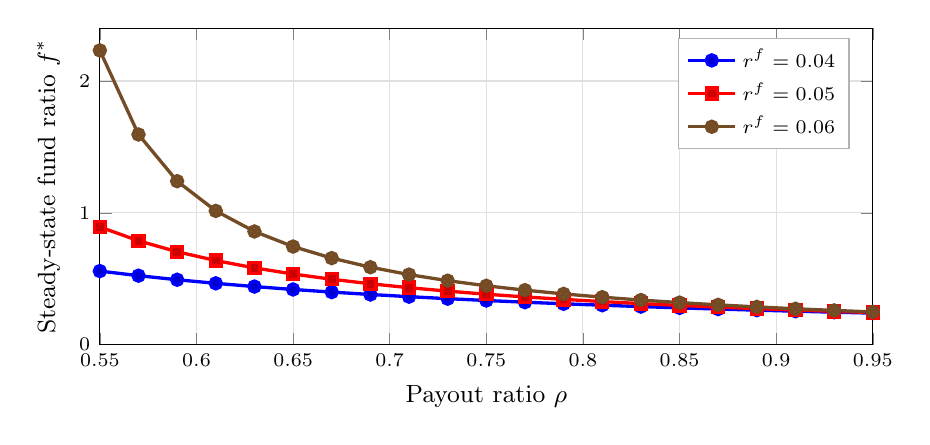
\begin{tikzpicture}
\begin{axis}[
  width=0.94\columnwidth, height=5.6cm,
  xlabel={Payout ratio $\rho$},
  ylabel={Steady-state fund ratio $f^{*}$},
  xmin=0.55, xmax=0.95, ymin=0, ymax=2.4,
  grid=major, grid style={black!12},
  legend pos=north east, legend cell align=left,
  legend style={font=\scriptsize, draw=black!30},
  label style={font=\small}, tick label style={font=\scriptsize},
  every axis plot/.append style={very thick, mark=none}
]
\addplot coordinates {(0.550,0.55792) (0.570,0.52305) (0.590,0.49228) (0.610,0.46493) (0.630,0.44046) (0.650,0.41844) (0.670,0.39851) (0.690,0.38040) (0.710,0.36386) (0.730,0.34870) (0.750,0.33475) (0.770,0.32187) (0.790,0.30995) (0.810,0.29888) (0.830,0.28858) (0.850,0.27896) (0.870,0.26996) (0.890,0.26152) (0.910,0.25360) (0.930,0.24614) (0.950,0.23911)};
\addlegendentry{$r^{f}=0.04$}
\addplot coordinates {(0.550,0.89267) (0.570,0.78765) (0.590,0.70474) (0.610,0.63762) (0.630,0.58217) (0.650,0.53560) (0.670,0.49593) (0.690,0.46172) (0.710,0.43194) (0.730,0.40576) (0.750,0.38257) (0.770,0.36189) (0.790,0.34333) (0.810,0.32659) (0.830,0.31140) (0.850,0.29756) (0.870,0.28489) (0.890,0.27327) (0.910,0.26255) (0.930,0.25264) (0.950,0.24345)};
\addlegendentry{$r^{f}=0.05$}
\addplot coordinates {(0.550,2.23167) (0.570,1.59405) (0.590,1.23981) (0.610,1.01439) (0.630,0.85833) (0.650,0.74389) (0.670,0.65637) (0.690,0.58728) (0.710,0.53135) (0.730,0.48514) (0.750,0.44633) (0.770,0.41327) (0.790,0.38477) (0.810,0.35995) (0.830,0.33813) (0.850,0.31881) (0.870,0.30158) (0.890,0.28611) (0.910,0.27215) (0.930,0.25950) (0.950,0.24796)};
\addlegendentry{$r^{f}=0.06$}
\end{axis}
\end{tikzpicture}
\caption{Steady-state fund-to-output ratio $f^{*}$ from \eqref{eq:fstar} against the payout ratio $\rho$, for three real fund returns, with $g=0.03$ and inflow share $s=0.0065$. Each curve diverges as $\rho$ approaches the stability boundary $\rho = 1-g/r^{f}$ of \eqref{eq:stab}.}
\label{fig:fund}
\end{figure}

\begin{table}[!t]
\centering
\caption{Steady-state fund ratio $f^{*}$, per-capita dividend $d^{*}$ as a percentage of per-capita output, and convergence half-life, computed from Propositions~\ref{prop:fund}--\ref{prop:rg} with $g=0.03$ and $s=0.0065$. Values are analytically derived, not simulated. Note that $d^{*}$ falls as $\rho$ rises, consistent with Proposition~\ref{prop:rg} since $r^{f}>g$ throughout.}
\label{tab:fund}
\footnotesize
\begin{tabular}{@{}c c c c c@{}}
\toprule
$r^{f}$ & $\rho$ & $f^{*}$ & $d^{*}$ (\%) & Half-life (years) \\
\midrule
0.04 & 0.55 & 0.558 & 1.23 & 59.1 \\
0.04 & 0.75 & 0.335 & 1.00 & 35.3 \\
0.04 & 0.95 & 0.239 & 0.91 & 25.1 \\
\addlinespace
0.05 & 0.55 & 0.893 & 2.46 & 94.8 \\
0.05 & 0.75 & 0.383 & 1.44 & 40.4 \\
0.05 & 0.95 & 0.244 & 1.16 & 25.6 \\
\addlinespace
0.06 & 0.55 & 2.232 & 7.36 & 237.6 \\
0.06 & 0.75 & 0.446 & 2.01 & 47.2 \\
0.06 & 0.95 & 0.248 & 1.41 & 26.1 \\
\bottomrule
\end{tabular}
\end{table}

Inverting \eqref{eq:fstar} gives a direct design rule: to sustain a dividend equal to a share $\kappa_d$ of per-capita output, the required inflow is $s = \kappa_d[g-(1-\rho)r^{f}]/[\rho r^{f}(1+g)]$. For $\kappa_d = 0.02$, $r^{f}=0.05$, $\rho=0.60$ and $g=0.03$, this requires a steady-state fund of $66.7\%$ of output financed by an annual inflow of $0.65\%$ of output. Table~\ref{tab:fund} also records a finding that tempers the proposal: convergence is slow, with a half-life of roughly $71$ years under this calibration. Dividend adequacy in the first decades therefore depends on the direct-transfer channel rather than on fund returns, and the fund should be presented as an intergenerational instrument rather than a short-run income policy.

\subsection{Automation Ownership Units}

CivicDividendOS adds a predistribution mechanism rather than relying exclusively on ex post transfers. When a qualifying firm receives major public AI subsidies, public compute, exclusive public data access, or government procurement support, policy may require a small Automation Ownership Unit contribution $\mathrm{AOU}_i = \xi_i \cdot \mathrm{Equity}_i$, with the units entering the fund rather than individual government departments. The logic parallels a resource fund: the public contributes infrastructure, research, data, procurement demand, education, and legal institutions that help create private automation value, and may therefore hold a modest diversified claim on future returns. Because equity contributions are non-cash, they relax the inflow constraint in \eqref{eq:fstar} without increasing the current-year burden on firm liquidity, which is a distinct advantage over cash levies for capital-constrained entrants.

\section{Cross-Border Deployment Nexus}
\label{sec:nexus}

Cloud AI complicates conventional tax residence because an agent may be trained in one jurisdiction, owned in a second, hosted in a third, and economically deployed in a fourth. We therefore define, for entity $i$ and jurisdiction $j$,

\begin{equation}
\label{eq:nexus}
\mathrm{Nexus}_{ij} = w_1 U_{ij} + w_2 R_{ij} + w_3 P_{ij} + w_4 O_{ij},
\end{equation}

where $U_{ij}$, $R_{ij}$, $P_{ij}$ and $O_{ij}$ are jurisdiction $j$'s shares of entity $i$'s metered usage, revenue, users, and physical operations respectively, and $\sum_k w_k = 1$ with $w_k \ge 0$.

\begin{proposition}[Exhaustive apportionment]
\label{prop:nexus}
If each component is a share satisfying $\sum_j U_{ij} = \sum_j R_{ij} = \sum_j P_{ij} = \sum_j O_{ij} = 1$, then $\sum_j \mathrm{Nexus}_{ij} = 1$, and the apportioned liabilities $\SAC_{ij} = \mathrm{Nexus}_{ij}\SAC_i$ satisfy $\sum_j \SAC_{ij} = \SAC_i$ exactly.
\end{proposition}

\begin{proof}
Summing \eqref{eq:nexus} over $j$ gives $\sum_k w_k \cdot 1 = 1$; multiplying by $\SAC_i$ gives the second identity.
\end{proof}

Server location is deliberately excluded from \eqref{eq:nexus}, since it is the most cheaply relocated of the candidate factors and therefore the most exposed to profit shifting. Revenue apportionment can then follow verified economic deployment rather than infrastructure siting. We stress that this mechanism would require coordination with existing international corporate tax rules, in particular the OECD/G20 two-pillar framework \cite{OECDTwoPillar2021}, and is proposed as a research mechanism rather than a claim about current law. Robustness to strategic manipulation of the remaining four components is an open question that we do not resolve here.

\section{Distribution Waterfall and Annual Fiscal Cycle}
\label{sec:waterfall}

\subsection{Waterfall}

The complete distribution mechanism begins from the factor decomposition $Y = Y_H + Y_A + Y_R + Y_D + Y_K$, with private primary distribution $Y^{\mathrm{priv}} = W_H + \Pi_{O} + R_D + R_K$ unchanged. CivicDividendOS then introduces a secondary and ownership-based distribution in which households receive

\begin{align}
\label{eq:household}
Y_H^{\mathrm{fin}} =\;& W_H - \mathrm{Tax}_H + \mathrm{Shield}_H + \mathrm{Dividend}_H \nonumber\\
&+ \mathrm{Transition}_H + \mathrm{Services}_H,
\end{align}

while owners and the public sector respectively receive

\begin{align}
\label{eq:ownerpublic}
Y_O^{\mathrm{fin}} &= \Pi_O - \mathrm{CIT}_O - \SAC_O + \mathrm{PrivRet}_O, \nonumber\\
Y_P &= \mathrm{CIT} + \SAC + \mathrm{FundRet},
\end{align}

with $Y_P$ in \eqref{eq:ownerpublic} split among public services, human-capability investment, transition support, and citizen dividends. Annual distributable returns divide as $\mathrm{Dist}_t = D^{\mathrm{cit}}_t + D^{\mathrm{tr}}_t + D^{\mathrm{cap}}_t + D^{\mathrm{pub}}_t$, with the per-capita civic dividend $\mathrm{CADiv}_t = \rho D^{\mathrm{cit}}_t / N_t$ and transition support $\mathrm{WTI}_i = g(\mathrm{WageLoss}_i, \mathrm{Tenure}_i, \mathrm{Exposure}_i, \mathrm{Training}_i)$. The design preserves private profit incentives while creating a parallel public claim on part of the automation surplus. Fig.~\ref{fig:waterfall} traces a unit of value added through the full sequence.

\begin{figure}[!t]
\centering
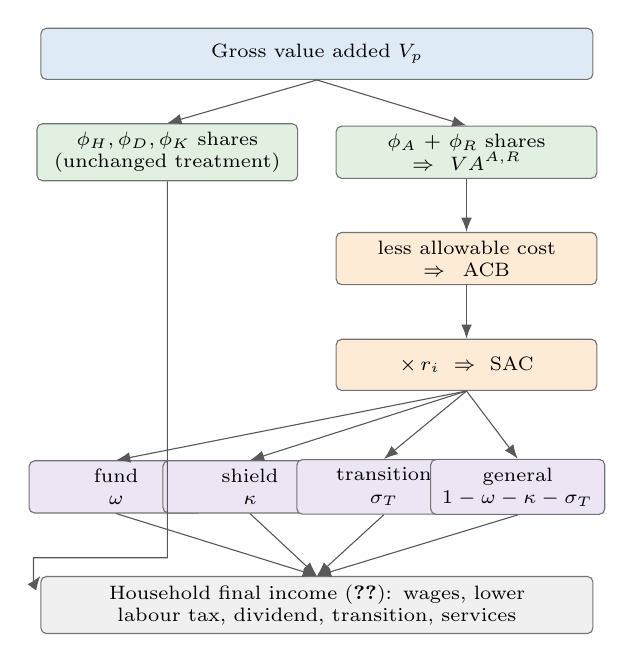
\begin{tikzpicture}[
  font=\scriptsize,
  n/.style={rounded corners=2pt, draw=black!55, align=center, inner sep=3pt, minimum height=6.5mm, text width=20mm},
  w/.style={n, text width=68mm},
  m/.style={n, text width=31mm},
  a/.style={-{Latex[length=1.8mm]}, draw=black!65}
]
\node[w, fill=cdMeasure] (v) at (0,0) {Gross value added $V_p$};
\node[m, fill=cdAttrib] (hdk) at (-1.9,-1.25) {$\phi_H,\phi_D,\phi_K$ shares\\(unchanged treatment)};
\node[m, fill=cdAttrib] (ar) at (1.9,-1.25) {$\phi_A + \phi_R$ shares\\$\Rightarrow VA^{A,R}$};
\node[m, fill=cdAssess] (acb2) at (1.9,-2.6) {less allowable cost\\$\Rightarrow \ACB$};
\node[m, fill=cdAssess] (sac2) at (1.9,-3.95) {$\times\, r_i \Rightarrow \SAC$};
\node[n, fill=cdDistrib] (om) at (-2.55,-5.5) {fund\\$\omega$};
\node[n, fill=cdDistrib] (ka) at (-0.85,-5.5) {shield\\$\kappa$};
\node[n, fill=cdDistrib] (tr) at (0.85,-5.5) {transition\\$\sigma_T$};
\node[n, fill=cdDistrib] (ge) at (2.55,-5.5) {general\\$1-\omega-\kappa-\sigma_T$};
\node[w, fill=cdGov] (out) at (0,-7.0) {Household final income \eqref{eq:household}: wages, lower labour tax, dividend, transition, services};
\draw[a] (v.south) -- (hdk.north);
\draw[a] (v.south) -- (ar.north);
\draw[a] (ar) -- (acb2);
\draw[a] (acb2) -- (sac2);
\draw[a] (sac2.south) -- (om.north);
\draw[a] (sac2.south) -- (ka.north);
\draw[a] (sac2.south) -- (tr.north);
\draw[a] (sac2.south) -- (ge.north);
\draw[a] (hdk.south) |- (-3.6,-6.4) -- (-3.6,-6.75) -- (out.north west);
\draw[a] (om.south) -- (out.north);
\draw[a] (ka.south) -- (out.north);
\draw[a] (tr.south) -- (out.north);
\draw[a] (ge.south) -- (out.north);
\end{tikzpicture}
\caption{Distribution waterfall. Only the attributed AI and robotic shares enter the contribution base; human, data, and conventional capital shares retain their existing fiscal treatment. Shares satisfy $\omega+\kappa+\sigma_T \le 1$ by Proposition~\ref{prop:shield}.}
\label{fig:waterfall}
\end{figure}

\subsection{Annual Fiscal Cycle}

Algorithm~\ref{alg:cycle} states the operational cycle. Steps 2--4 are the measurement and attribution layers, steps 5--8 the assessment layer, and steps 9--12 distribution and governance. The cycle is deliberately annual: the digital twin proposes a revised policy vector, but adoption requires the publication and oversight step described in Section~\ref{sec:twin}.

\begin{algorithm}[!t]
\caption{CivicDividendOS annual fiscal cycle}
\label{alg:cycle}
\begin{algorithmic}[1]
\Require Registry $\{\AEAP_j\}$, episodes $\{\mathcal{P}_i\}$, policy vector $\Theta$
\Ensure Liabilities $\{\SAC_{ij}\}$, fund state $F_{t+1}$, distributions
\State Refresh registry: validate owner, jurisdiction, task class, resources
\ForAll{episodes $p \in \bigcup_i \mathcal{P}_i$}
  \State Estimate coalition values $v_p(S)$ for all $S\subseteq\mathcal{F}$
  \State Compute Shapley shares $\phi_{p,f}$ by \eqref{eq:shapley}; post to ledger
  \State Assign mode $Z_p$ and episode scores
\EndFor
\ForAll{entities $i$}
  \State Aggregate $VA^{A,R}_i$; form indices $S_i, A^{\mathrm{aug}}_i, \dots$
  \State $\ACB_i \gets VA^{A,R}_i - C^{\mathrm{all}}_i$ \Comment{Eq.~\eqref{eq:acb}}
  \State $r_i \gets \clip(\tilde r_i, r_{\min}, r_{\max})$; $\SAC_i \gets r_i \ACB_i$
  \State Apportion $\SAC_{ij} \gets \mathrm{Nexus}_{ij}\SAC_i$ \Comment{Eq.~\eqref{eq:nexus}}
\EndFor
\State $\Rev_{\SAC} \gets \sum_{i,j}\SAC_{ij}$; verify $\omega + \kappa + \sigma_T \le 1$
\State Apply shield $\Delta\tau_L$ by \eqref{eq:shield}; disburse transition support
\State $F_{t+1} \gets F_t(1+r^{f}) + \omega\Rev_{\SAC} + E_t - \rho r^{f}F_t$
\State Distribute $\rho r^{f} F_t$ across the four channels
\State Twin proposes $\Theta'$; publish, review, and adopt or reject
\end{algorithmic}
\end{algorithm}

\section{Fiscal Digital Twin and Governance Safeguards}
\label{sec:twin}

Before changing rates or distribution shares, policy is screened in a fiscal digital twin containing heterogeneous households, firms, AI agents, robots, sectors, and jurisdictions, following the tradition of agent-based and learning-based fiscal policy design \cite{TaxAgent2025,Zheng2022AIEconomist}. The policy vector is $\Theta = \{r_0,\alpha,\beta,\gamma,\delta,\eta,\theta,\lambda,\mu,\nu,\omega,\rho,\kappa,\xi\}$, and the screening problem is the constrained scalarization

\begin{equation}
\label{eq:opt}
\Theta^{*} = \arg\max_{\Theta\in\mathcal{T}}\ \sum_{k} \omega_k\,\widetilde{U}_k(\Theta),
\end{equation}

subject to a revenue floor $\Rev(\Theta) \ge \underline{\Rev}$, an innovation floor $I(\Theta) \ge \underline{I}$, a leakage ceiling $L(\Theta) \le \overline{L}$, and the boundedness and feasibility constraints of Propositions~\ref{prop:bounded} and \ref{prop:shield}, where each $\widetilde{U}_k$ is a normalized outcome in growth, revenue, welfare, employment, innovation, inequality, and leakage, and the weights $\omega_k$ are published rather than inferred.

Two governance constraints on \eqref{eq:opt} are essential, and both are properties of the institution rather than of the model. First, the twin must report tax incidence explicitly, because a nominal contribution levied on an AI operator may ultimately fall on shareholders, workers, suppliers, or consumers, so policy cannot be evaluated from statutory rates alone. Second, the twin screens and proposes but does not autonomously set rates: adoption requires publication of $\Theta$, the weights $\omega_k$, and the simulation code; an appeal route for entities contesting their attribution or classification; and periodic external audit of the ledger. Without these constraints an adaptive fiscal system becomes an unaccountable one, and the transparency requirement is what distinguishes the proposal from automated rate setting.

\section{Worked Numerical Example}
\label{sec:example}

We trace a single entity end to end. An urban logistics company previously employing 100 human dispatchers and drivers introduces AI dispatch agents and autonomous delivery robots. A conventional tax system observes only lower payroll, fewer payroll contributions, higher firm profit, and larger investment in automated capital, and a simple robot tax would charge each robot a fixed annual amount irrespective of whether it replaced a worker, increased safety, or created new demand.

\subsection{Attribution}

Let annual value added be $V = 40.0$ monetary units (MU). To make the attribution reproducible rather than asserted, we specify the coalition value function explicitly as a game with pairwise complementarities,

\begin{equation}
\label{eq:game}
v(S) = \sum_{f\in S} a_f + \!\!\sum_{\{f,f'\}\subseteq S}\!\! b_{ff'},
\end{equation}

with singleton weights $a = (a_H,a_A,a_R,a_D,a_K) = (0.220, 0.135, 0.220, 0.020, 0.045)$ and pair weights $b_{HA}=0.10$, $b_{AD}=0.05$, $b_{RK}=0.06$, $b_{AR}=0.06$, $b_{HR}=0.04$, $b_{HK}=b_{AK}=0.02$, $b_{DK}=0.01$, normalized so that $v(\mathcal{F})=1$. The game \eqref{eq:game} is monotone, satisfying Assumption~\ref{as:mono}. For this class the Shapley value admits the closed form $\psi_f = a_f + \tfrac{1}{2}\sum_{f'} b_{ff'}$, since each singleton term accrues entirely to its factor and each pair term is split equally. Evaluating gives

\begin{equation}
\label{eq:shares}
\begin{split}
\phi_H = 0.30,\quad \phi_A = 0.25,\quad \phi_R = 0.30,\\
\phi_D = 0.05,\quad \phi_K = 0.10,
\end{split}
\end{equation}

which sum to unity as required by Proposition~\ref{prop:balance}. Summing the AI and robotic entries of \eqref{eq:shares}, the share of attributable value is $VA^{A,R} = 0.55V = 22.0$ MU. With allowable compute, energy, maintenance, and depreciation costs of $C^{\mathrm{all}} = 8.4$ MU, the base is $\ACB = 13.6$ MU.

\subsection{Rate and Liability}

Table~\ref{tab:example} lists the calibration. In the substitution-intensive configuration the raw score is $\tilde r = 0.116$, which lies inside $[r_{\min},r_{\max}]$ so $r = 0.116$ and $\SAC = 1.578$ MU. In an augmentation-intensive counterfactual with the same base, in which substitution falls to $S = 0.15$, displacement to $E^{\mathrm{disp}} = 0.10$ and augmentation rises to $A^{\mathrm{aug}} = 0.85$, the raw score falls to $\tilde r = 0.0095$ and the liability to $0.129$ MU. The same firm with the same automation value added thus faces a liability differing by a factor of $12.2$ depending on measured effect on human work, which is precisely the discrimination a fixed robot tax cannot express: a levy of $0.004$ MU on each of 60 robots yields $0.240$ MU in both configurations. (Annual value added in this example is $V = 40.0$ MU, so the monetary unit is not millions; an earlier version of this example stated the per-robot levy in units inconsistent with $V$.)

\begin{table}[!t]
\centering
\caption{Calibration and results for the worked example of Section~\ref{sec:example}. Indices and weights are illustrative policy settings; the resulting liabilities follow deterministically from \eqref{eq:rawrate}--\eqref{eq:rate}.}
\label{tab:example}
\footnotesize
\begin{tabular}{@{}l c c@{}}
\toprule
\textbf{Quantity} & \textbf{Substitution} & \textbf{Augmentation} \\
\midrule
\multicolumn{3}{@{}l}{\textit{Rate weights}} \\
$r_0$; $r_{\min}$; $r_{\max}$ & \multicolumn{2}{c}{$0.08$; $0.00$; $0.25$} \\
$\alpha,\beta,\gamma,\delta,\eta$ & \multicolumn{2}{c}{$0.10, 0.06, 0.05, 0.04, 0.05$} \\
$\theta,\lambda,\mu,\nu$ & \multicolumn{2}{c}{$0.09, 0.07, 0.05, 0.06$} \\
\addlinespace
\multicolumn{3}{@{}l}{\textit{Indices}} \\
$S_i$ & 0.62 & 0.15 \\
$C^{\mathrm{rent}}_i$ & 0.35 & 0.35 \\
$E^{\mathrm{disp}}_i$ & 0.48 & 0.10 \\
$X^{\mathrm{ext}}_i$; $R^{\mathrm{rev}}_i$ & 0.10; 0.55 & 0.10; 0.55 \\
$A^{\mathrm{aug}}_i$ & 0.40 & 0.85 \\
$T^{\mathrm{train}}_i$; $B^{\mathrm{broad}}_i$; $N^{\mathrm{new}}_i$ & 0.55; 0.20; 0.30 & 0.55; 0.20; 0.30 \\
\addlinespace
\multicolumn{3}{@{}l}{\textit{Outcome}} \\
$\ACB$ (MU) & 13.60 & 13.60 \\
$\tilde r_i$ & 0.1160 & 0.0095 \\
$r_i$ & 0.1160 & 0.0095 \\
$\SAC_i$ (MU) & 1.578 & 0.129 \\
Fixed robot tax (MU) & 0.240 & 0.240 \\
\bottomrule
\end{tabular}
\end{table}

\subsection{Allocation}

Revenue is not paid by the robots but by the firm that owns or beneficially uses the automation. With $\omega = 0.40$, $\kappa = 0.25$, $\sigma_T = 0.15$ and a general-revenue residual of $0.20$, satisfying the feasibility condition of Proposition~\ref{prop:shield}, the substitution-case liability of $1.578$ MU allocates to $0.631$ MU into the fund, $0.394$ MU to the earned-income shield, $0.237$ MU to immediate transition insurance, and $0.316$ MU to general revenue. The long-run allocation is therefore that humans receive wages plus a lower labour tax plus a dividend, owners receive profit net of corporate tax and the contribution plus their private return, the public receives the contribution plus public equity returns, and future workers receive the human-capability endowment.

\section{Evaluation Protocol and Reproducibility}
\label{sec:eval}

\subsection{Testbed and Baselines}

The framework should be evaluated in a heterogeneous-agent macroeconomic and urban-production simulation containing households differing in income, skills, wealth, and automation exposure; firms with heterogeneous productivity and market power; conventional, AI-agent, and robotic capital; government tax and transfer accounts; a public automation wealth fund; and multiple domestic and cross-border sectors. Table~\ref{tab:config} states the configuration used.

\begin{table}[!t]
\centering
\caption{Proposed evaluation testbed configuration. These are the settings actually used to produce Table~\ref{tab:results}.}
\label{tab:config}
\footnotesize
\begin{tabular}{@{}l l@{}}
\toprule
\textbf{Dimension} & \textbf{Setting} \\
\midrule
Households & 10{,}000; lognormal skill and wealth, exposure \\
 & negatively correlated with skill \\
Firms & 500; lognormal productivity, beta labour weight \\
Factors & Labour $L$ and a composite machine factor $M$ \\
Production & CES in $(L,M)$, $\sigma=1.5$, span of control $\gamma=0.85$ \\
Driver & Machine price falls $0.6\%$ per quarter \\
Labour supply & Elasticity $\varepsilon_L=0.30$ to the net-of-tax wage \\
Jurisdictions & 1 (the nexus rule of Sec.~\ref{sec:nexus} is not exercised) \\
Horizon & 200 quarters (50 years) plus 40-quarter burn-in \\
Replications & 50 seeds per arm; common random numbers \\
Attribution & Exact Shapley over $\{L,M\}$, $\psi_L+\psi_M=Y_f$ \\
Deduction share & $\varphi=1$ (arm B6), $\varphi=1/2$ (arm B6c) \\
Budget rule & $\tau_L$ clears the budget; spending fixed at $35\%$ of $Y$ \\
Uncertainty & Paired bootstrap 95\% CIs over seeds, 2000 resamples \\
\bottomrule
\end{tabular}
\end{table}

CivicDividendOS should be compared against seven arms: (B0) the existing labour and capital tax system, (B1) a fixed robot tax, (B2) a broad capital-income tax increase, (B3) UBI funded through general taxation, (B4) an automation tax plus targeted retraining, (B5) a sovereign or public wealth fund without factor-origin taxation, and (B6) the integrated framework proposed here, which we run in two variants distinguished only by the cost-deduction share of Proposition~\ref{prop:margin}: B6 with the base exactly as specified and B6c with the corrected base. Every arm finances the same baseline public spending, but the arms are \emph{not} revenue-matched: each also finances its own programme spending, so total spending differs across arms by up to two percentage points of output. Contrasts therefore reflect fiscal stance as well as instrument design, and the revenue-normalised comparison of Section~\ref{sec:results} is the one to read when ranking instruments.

\subsection{Model Specification}
\label{sec:model}

The testbed is a discrete-time model of $N_F = 500$ heterogeneous firms and $N_H = 10{,}000$ heterogeneous households run at quarterly frequency for $40$ burn-in and $200$ reported quarters. Firm $f$ produces $Y_f = A_f X_f^{\gamma}$ with $X_f = [\alpha_f L_f^{\varrho} + (1-\alpha_f)M_f^{\varrho}]^{1/\varrho}$, where $M$ denotes combined AI-agent and robotic services, $\sigma = 1/(1-\varrho) = 1.5$ is the elasticity of substitution between labour and machines, and $\gamma = 0.85$ gives decreasing returns and hence positive pure profit. Productivity $A_f$ and the labour weight $\alpha_f$ are drawn from lognormal and beta distributions respectively, and firms take the wage $w$ and the machine price $p_M$ as given. The machine price falls at $0.6\%$ per quarter, which is the single exogenous driver of the transition.

Households differ in skill, initial wealth, and automation exposure, with exposure negatively correlated with skill. Labour is supplied in efficiency units with elasticity $\varepsilon_L = 0.30$ with respect to the net-of-tax wage, and the wage clears the labour market each quarter. Households whose exposure is high lose efficiency units as automation advances, at rate $\lambda_d$ per unit of exposure and adoption growth, which is the model's displacement channel; retraining expenditure restores efficiency units in proportion to exposure. Savings rates rise with the wealth rank, which generates a wealth distribution substantially more unequal than the income distribution.

Two features are essential to interpreting the results. First, the model implements the paper's own attribution rule rather than a proxy for it: $\psi_M$ is computed exactly from \eqref{eq:shapley} for the two-factor game, so $\psi_L + \psi_M = Y_f$ holds identically and the contribution base is the attributed automation value added net of the admitted share $\varphi$ of machine cost. Second, every arm finances an identical path of baseline public spending, fixed at $35\%$ of output, plus its own programme spending, with the labour income tax adjusting each quarter to clear the government budget. The labour tax rate is therefore an \emph{outcome} rather than a parameter, and the Human Earned-Income Shield of Section~\ref{sec:recycle} appears in the results as the reduction in the labour tax that automation revenue makes possible. Arms therefore differ both in the instruments used and in how much revenue those instruments raise, which is why output effects alone do not rank them.

The arms are those of Section~\ref{sec:eval}, with arm B6 split into two variants that differ only in the cost-deduction share of Proposition~\ref{prop:margin}: B6 uses the base exactly as specified in \eqref{eq:acb} with $\varphi = 1$, and B6c uses the corrected base with $\varphi = 1/2$. Arms B1 and B4 levy a genuine wedge on the machine price, whereas B6 and B6c levy the contribution on the base $\ACB$, whose marginal effect on the machine decision is $r_i\,\partial\ACB/\partial M$ by Proposition~\ref{prop:margin}. All arms share common random numbers across $50$ seeds, so contrasts are paired and confidence intervals are computed by bootstrap over seeds.

\subsection{Metrics}

The metrics reported in Table~\ref{tab:results} are output, hours, the terminal labour share, income and wealth Gini coefficients, the poverty rate, the labour tax rate required to clear the budget, the fund-to-output ratio, and the per-capita dividend. A full study should additionally report: GDP and productivity; AI and robot adoption; employment and hours; wage share and capital share; household disposable income; income and wealth Gini coefficients; poverty rate; revenue volatility; payroll and social-insurance funding; investment and innovation; firm entry and exit; public-fund value; citizen dividend per capita; worker-transition duration; human-capability investment; tax avoidance and leakage; and intergenerational wealth distribution. Sensitivity analysis should vary AI and robot costs, substitution elasticities, market concentration, international capital mobility, tax compliance, and the speed of technological progress. Effects should be reported with uncertainty, in the form $\Delta\mathrm{Gini} = -0.044$, $\mathrm{CI}_{95\%} = [-0.058, -0.031]$, rather than as point estimates.

% === RESULTS SECTION REVISED POST-AUDIT ===
\subsection{Results}
\label{sec:results}

Table~\ref{tab:results} reports the campaign and Table~\ref{tab:ci} the paired
contrasts. All numerical entries in these tables are generated directly from the
simulation output by \texttt{scripts/make\_tables.py} and included with
\verb|\input|; none is transcribed by hand.

Two framing points come first, because they govern how everything below should
be read.

\emph{The confidence intervals are replication intervals.} Arms share common
random numbers, so contrasts are paired and the bootstrap intervals over seeds
are extremely tight. That is a statement about the reproducibility of the
simulation at one parameter vector, and not about the certainty of any policy
conclusion. The sensitivity analysis of Section~\ref{sec:sensitivity} moves the
central estimate by tens of percentage points, which no replication interval
here can see.

\emph{The arms are not revenue-matched.} Each finances the same baseline public
spending plus its own programme, so total spending differs across arms. Ranking
instruments by output effect alone is therefore not valid, and
Table~\ref{tab:revnorm} gives the revenue-normalised comparison.

Six findings stand out, and they do not uniformly favour the proposed framework.

First, the fixed robot tax of arm B1 is by a wide margin the most costly
instrument in output terms, at $-6.12\%$ relative to baseline, while raising
$1.91\%$ of output in revenue. It does support the labour share, which ends at
$0.341$ against $0.298$ in the baseline, but it achieves this by taxing an input
at a uniform rate irrespective of whether the automation in question displaced
anyone. This is the quantitative counterpart of the attribution gap of
Section~\ref{sec:problem}.

Second, the framework as literally specified in \eqref{eq:acb} is close to
inert. Arm B6 raises only $0.24\%$ of output and reduces the income Gini by
$0.0022$, which is statistically clear and economically negligible. Its output
effect is positive, at $+2.45\%$, \emph{precisely because} the base is
marginally subsidising in the sense of Proposition~\ref{prop:margin}. A positive
output number here is evidence of the design defect, not of merit.

Third, the corrected base repairs the revenue problem but does not deliver
dominance. Arm B6c raises $0.88\%$ of output, lowers the required labour tax
from $0.381$ to $0.370$ $(\Delta\tau_L = -0.0111$, $\mathrm{CI}_{95\%} =
[-0.0118,-0.0103])$, reduces the income Gini by $0.0072$ $(\mathrm{CI}_{95\%} =
[-0.0077,-0.0068])$, and raises output by $3.18\%$ and labour demand in
efficiency units by $6.78\%$, holding the terminal labour share at $0.316$
against $0.298$. These figures are produced under corrected budget accounting,
in which the full contribution liability $r_i\ACB_i$ is debited from firm
profit while the marginal decision price remains $p_M + r_i\,\partial\ACB/
\partial M$ as Proposition~\ref{prop:margin} requires. Under the earlier
accounting, in which only the marginal wedge was debited, the same arm showed
$+3.30\%$; the difference is the mechanical effect of charging the
inframarginal liability to somebody.

Fourth, and decisively against the strong reading of the proposal, B6c is
\emph{not} the most efficient instrument once revenue is held constant.
Table~\ref{tab:revnorm} reports revenue raised per unit of deadweight loss on
the labour margin. B6c returns $0.45$, against $1.47$ for the fixed robot tax
of B1 and $0.89$ for the automation levy of B4. B6c looks good on output
largely because it raises little revenue. Furthermore, arm B9, which finances
the same programme with a lump-sum levy rather than with the attributed
contribution, attains $+3.03\%$ output against B6c's $+3.18\%$. Most of the
output advantage is therefore a fiscal-stance effect rather than a return to
the attribution machinery, which is the central claim the framework needs and
does not establish here.

Fifth, targeted transfers remain the better instrument for near-term
distributional objectives. Arm B3 attains the lowest income Gini at $0.3147$ and
much the lowest poverty rate at $9.95\%$, outcomes that B6c does not approach,
and it does so immediately rather than over decades. The cost is the highest
labour tax of any arm at $0.413$. A fund whose half-life is measured in decades
cannot substitute for transfers within a political cycle: the dividend in B6c
reaches only $0.26\%$ of output after fifty years.

Sixth, arm B4, a flat automation levy recycled into retraining, delivers the
largest gain in labour demand of any arm, at $+8.52\%$ in efficiency units, for
an output cost of only $-0.72\%$. Much of the benefit attributed to the
attribution machinery can be obtained by a simpler instrument coupled to an
active labour-market policy.

\emph{A note on the employment column.} The quantity reported here is aggregate
labour demand measured in \emph{efficiency units}, $\sum_f L_f$. It is not hours
and it is not employment. A worker whose efficiency has been reduced by
displacement contributes less to it while remaining fully employed, and
retraining expenditure raises it directly. The model has no extensive
employment margin --- labour supply is a smooth function of the net-of-tax wage
and no agent is ever unemployed --- so it cannot speak to employment in the
ordinary sense. Table~\ref{tab:employment} reports efficiency units, a headcount
above the displacement floor, and the wage separately.

% GENERATED FILE -- do not edit by hand.
% Written by scripts/make_tables.py from results/raw/main.json
% git 8f6da5f (dirty)
B0 & Existing labour/capital tax system & $+0.00$ & $+0.00$ & $0.298$ & $0.3296$ & $0.5575$ & $0.381$ & $0.00$ & $0.00$ \\
B1 & Fixed robot tax & $-6.12$ & $+3.34$ & $0.341$ & $0.3245$ & $0.5558$ & $0.325$ & $0.00$ & $0.00$ \\
B2 & Broad capital-income tax increase & $+0.84$ & $+1.20$ & $0.298$ & $0.3255$ & $0.5535$ & $0.356$ & $0.00$ & $0.00$ \\
B3 & UBI via general taxation & $-1.05$ & $-1.55$ & $0.297$ & $0.3147$ & $0.5569$ & $0.413$ & $0.00$ & $0.00$ \\
B4 & Automation tax plus retraining & $-0.72$ & $+8.52$ & $0.338$ & $0.3247$ & $0.5556$ & $0.352$ & $0.00$ & $0.00$ \\
B5 & Public wealth fund, no factor-origin tax & $-0.10$ & $-0.14$ & $0.298$ & $0.3283$ & $0.5575$ & $0.384$ & $0.07$ & $0.17$ \\
B6 & CivicDividendOS, base as specified & $+2.45$ & $+1.56$ & $0.297$ & $0.3274$ & $0.5569$ & $0.385$ & $0.04$ & $0.08$ \\
B6c & \textbf{CivicDividendOS (corrected base)} & $+3.18$ & $+6.78$ & $0.316$ & $0.3224$ & $0.5558$ & $0.370$ & $0.15$ & $0.26$ \\
B7 & Optimal linear capital tax & $+0.41$ & $+0.60$ & $0.298$ & $0.3275$ & $0.5555$ & $0.369$ & $0.00$ & $0.00$ \\
B8 & Consumption-tax shift & $+1.01$ & $+1.45$ & $0.299$ & $0.3282$ & $0.5562$ & $0.350$ & $0.00$ & $0.00$ \\
B9 & Lump-sum-financed CivicDividendOS & $+3.03$ & $+2.38$ & $0.298$ & $0.3351$ & $0.5573$ & $0.368$ & $0.04$ & $0.08$ \\
B10 & EITC-style wage subsidy & $-0.23$ & $-0.35$ & $0.298$ & $0.3213$ & $0.5569$ & $0.389$ & $0.00$ & $0.00$ \\
B11 & CivicDividendOS with full deduction (phi = 0) & $-3.13$ & $+2.07$ & $0.319$ & $0.3255$ & $0.5559$ & $0.345$ & $0.00$ & $0.00$ \\
B12 & Thuemmel-style optimal robot tax & $-2.54$ & $+1.34$ & $0.313$ & $0.3275$ & $0.5568$ & $0.359$ & $0.00$ & $0.00$ \\

% GENERATED FILE -- do not edit by hand.
% Written by scripts/make_tables.py from results/raw/main.json
% git bec4745 (dirty)
\begin{table}[!t]
\centering
\caption{Paired differences against arm B0 with bootstrap 95\% confidence intervals over 50 seeds (2000 resamples). These are \emph{replication} intervals: they quantify Monte-Carlo variation at one fixed parameter vector and say nothing about parameter uncertainty. See Section~\ref{sec:sensitivity}.}
\label{tab:ci}
\scriptsize
\begin{tabular}{@{}l c c c c@{}}
\toprule
\textbf{Arm} & $\Delta$\textbf{Gini} & \textbf{95\% CI} & $\Delta\tau_L$ & \textbf{95\% CI} \\
\midrule
B1 & $-0.0051$ & $[-0.0056, -0.0046]$ & $-0.0558$ & $[-0.0577, -0.0537]$ \\
B2 & $-0.0042$ & $[-0.0044, -0.0039]$ & $-0.0257$ & $[-0.0262, -0.0252]$ \\
B3 & $-0.0149$ & $[-0.0154, -0.0145]$ & $+0.0322$ & $[+0.0315, +0.0329]$ \\
B4 & $-0.0050$ & $[-0.0053, -0.0046]$ & $-0.0288$ & $[-0.0296, -0.0278]$ \\
B5 & $-0.0013$ & $[-0.0013, -0.0013]$ & $+0.0029$ & $[+0.0028, +0.0030]$ \\
B6 & $-0.0022$ & $[-0.0023, -0.0021]$ & $+0.0033$ & $[+0.0032, +0.0034]$ \\
B6c & $-0.0072$ & $[-0.0077, -0.0068]$ & $-0.0111$ & $[-0.0118, -0.0103]$ \\
B7 & $-0.0022$ & $[-0.0023, -0.0021]$ & $-0.0127$ & $[-0.0129, -0.0125]$ \\
B8 & $-0.0014$ & $[-0.0015, -0.0014]$ & $-0.0310$ & $[-0.0315, -0.0304]$ \\
B9 & $+0.0055$ & $[+0.0053, +0.0056]$ & $-0.0137$ & $[-0.0140, -0.0134]$ \\
B10 & $-0.0083$ & $[-0.0084, -0.0083]$ & $+0.0075$ & $[+0.0073, +0.0077]$ \\
B11 & $-0.0041$ & $[-0.0046, -0.0037]$ & $-0.0360$ & $[-0.0377, -0.0343]$ \\
B12 & $-0.0022$ & $[-0.0023, -0.0020]$ & $-0.0220$ & $[-0.0225, -0.0214]$ \\
\bottomrule
\end{tabular}
\end{table}

% GENERATED FILE -- do not edit by hand.
% Written by scripts/make_tables.py from results/raw/main.json
% git 8f6da5f (dirty)
B0 & $+0.00$ & $0.000$ & $2.307$ & $0.000$ \\
B1 & $-6.12$ & $1.907$ & $1.488$ & $1.472$ \\
B2 & $+0.84$ & $0.000$ & $1.954$ & $0.000$ \\
B3 & $-1.05$ & $0.000$ & $2.789$ & $0.000$ \\
B4 & $-0.72$ & $1.476$ & $1.924$ & $0.892$ \\
B5 & $-0.10$ & $0.000$ & $2.355$ & $0.000$ \\
B6 & $+2.45$ & $0.238$ & $2.352$ & $0.109$ \\
B6c & $+3.18$ & $0.877$ & $2.186$ & $0.451$ \\
B7 & $+0.41$ & $0.000$ & $2.129$ & $0.000$ \\
B8 & $+1.01$ & $0.000$ & $1.885$ & $0.000$ \\
B9 & $+3.03$ & $0.239$ & $2.113$ & $0.123$ \\
B10 & $-0.23$ & $0.000$ & $2.404$ & $0.000$ \\
B11 & $-3.13$ & $1.486$ & $1.783$ & $0.941$ \\
B12 & $-2.54$ & $0.800$ & $1.974$ & $0.472$ \\

% GENERATED FILE -- do not edit by hand.
% Written by scripts/make_tables.py from results/raw/main.json
% git 08de3bc (dirty)
\begin{table}[!t]
\centering
\caption{Labour-market quantities, separated. Efficiency units are aggregate labour demand $\sum_f L_f$; headcount counts workers above the displacement floor. The model has no extensive employment margin --- labour supply is a smooth function of the net-of-tax wage and no agent is ever unemployed --- so neither column is an unemployment rate, and the quantity reported as ``Hours'' in an earlier version of this table was the first of these.}
\label{tab:employment}
\scriptsize
\begin{tabular}{@{}l c c c c c@{}}
\toprule
\textbf{Arm} & \textbf{Eff. units} & $\Delta$\textbf{(\%)} & \textbf{Headcount} & $\Delta$\textbf{(\%)} & \textbf{Wage} \\
\midrule
B0 & $6470.0$ & $+0.00$ & $10000.0$ & $+0.00$ & $0.4980$ \\
B1 & $6685.2$ & $+3.34$ & $10000.0$ & $+0.00$ & $0.4842$ \\
B2 & $6547.9$ & $+1.20$ & $10000.0$ & $+0.00$ & $0.4968$ \\
B3 & $6369.9$ & $-1.55$ & $10000.0$ & $+0.00$ & $0.4995$ \\
B4 & $7020.0$ & $+8.52$ & $10000.0$ & $+0.00$ & $0.4816$ \\
B5 & $6460.8$ & $-0.14$ & $10000.0$ & $+0.00$ & $0.4981$ \\
B6 & $6570.8$ & $+1.56$ & $10000.0$ & $+0.00$ & $0.4979$ \\
B6c & $6907.9$ & $+6.78$ & $10000.0$ & $+0.00$ & $0.4897$ \\
B7 & $6508.7$ & $+0.60$ & $10000.0$ & $+0.00$ & $0.4974$ \\
B8 & $6563.7$ & $+1.45$ & $10000.0$ & $+0.00$ & $0.4965$ \\
B9 & $6624.2$ & $+2.38$ & $10000.0$ & $+0.00$ & $0.4971$ \\
B10 & $6447.4$ & $-0.35$ & $10000.0$ & $+0.00$ & $0.4983$ \\
B11 & $6603.5$ & $+2.07$ & $10000.0$ & $+0.00$ & $0.4920$ \\
B12 & $6556.3$ & $+1.34$ & $10000.0$ & $+0.00$ & $0.4924$ \\
\bottomrule
\end{tabular}
\end{table}

% GENERATED FILE -- do not edit by hand.
% Written by scripts/make_tables.py from results/raw/main.json
% git 8f6da5f (dirty)
B1 & $76.3$ & $23.7$ & $1.907$ \\
B4 & $76.1$ & $23.9$ & $1.476$ \\
B6 & $76.6$ & $23.4$ & $0.238$ \\
B6c & $76.7$ & $23.3$ & $0.877$ \\
B9 & $76.6$ & $23.4$ & $0.239$ \\
B11 & $77.0$ & $23.0$ & $1.486$ \\
B12 & $75.2$ & $24.8$ & $0.800$ \\


\subsection{Sensitivity and the Region of Validity}
\label{sec:sensitivity}

The results of Section~\ref{sec:results} are computed at a single point,
$\sigma = 1.5$ and $\gamma = 0.85$. Neither parameter is calibrated, and the
Metrics discussion of Section~\ref{sec:eval} requires that sensitivity to them
be reported. We therefore sweep both.

Table~\ref{tab:sigmagamma} reports arm B6c's output effect across
$\sigma \in \{1.2, 1.5, 2.0, 3.0, 5.0, 8.0\}$ and
$\gamma \in \{0.75, 0.85, 0.95\}$, at ten seeds per cell under common random
numbers.

\textbf{The output advantage is positive in only four of the eighteen cells.}
At $\gamma = 0.85$ it is $+4.78\%$ at $\sigma = 1.2$ and $+3.01\%$ at
$\sigma = 1.5$, but $-2.23\%$ at $\sigma = 2.0$ and $-24.99\%$ at
$\sigma = 8.0$. The sign therefore reverses between $\sigma = 1.5$ and
$\sigma = 2.0$, and the region in which the advantage holds is approximately
$\sigma \lesssim 1.7$ at $\gamma = 0.85$. Since the empirical literature places
the labour--capital elasticity of substitution across a range that comfortably
spans this boundary, \textbf{the result must be read as conditional on a low
elasticity and not as a general property of the instrument}. At
$\gamma = 0.95$, close to constant returns, firm scale becomes explosive and the
model is better regarded as outside its domain of validity than as delivering a
policy result; that row is reported as a boundary diagnostic.

The same sweep clarifies Proposition~\ref{prop:margin}. Arm B6, with full
deduction, shows a small positive output effect almost everywhere in the grid,
which is exactly what a marginally subsidising base predicts. The proposition is
therefore supported by the sweep, while the proposal's headline advantage is
not.

% GENERATED FILE -- do not edit by hand.
% Written by scripts/make_tables.py from results/raw/E01.json
% git 08de3bc (dirty)
\begin{table}[!t]
\centering
\caption{Sensitivity of the output effect to the elasticity of substitution $\sigma$ and the span of control $\gamma$, ten seeds per cell under common random numbers, with $\rho = 1-1/\sigma$. The $\gamma>\rho$ column records whether the marginal-incidence inequality of Proposition~\ref{prop:margin} holds identically. \textbf{Arm B6c's advantage is positive in only four of the eighteen cells, and the sign reverses between $\sigma=1.5$ and $\sigma=2.0$ at $\gamma=0.85$.} The $\gamma=0.95$ row is a boundary diagnostic: near constant returns firm scale becomes explosive and the model is outside its domain of validity.}
\label{tab:sigmagamma}
\scriptsize
\begin{tabular}{@{}c c c c c c c@{}}
\toprule
$\sigma$ & $\gamma$ & $\rho$ & $\gamma>\rho$ & \textbf{B6 (\%)} & \textbf{B6c (\%)} & \textbf{B6c 95\% CI} \\
\midrule
$1.2$ & $0.75$ & $0.167$ & yes & $+3.37$ & $+3.29$ & $[+3.21, +3.38]$ \\
$1.2$ & $0.85$ & $0.167$ & yes & $+3.44$ & $+4.56$ & $[+4.23, +4.82]$ \\
$1.2$ & $0.95$ & $0.167$ & yes & $+5.99$ & $-0.36$ & $[-3.53, +2.26]$ \\
$1.5$ & $0.75$ & $0.333$ & yes & $+2.01$ & $+2.32$ & $[+2.24, +2.40]$ \\
$1.5$ & $0.85$ & $0.333$ & yes & $+2.40$ & $+2.81$ & $[+1.83, +3.48]$ \\
$1.5$ & $0.95$ & $0.333$ & yes & $+2.22$ & $-48.87$ & $[-55.75, -41.92]$ \\
$2.0$ & $0.75$ & $0.500$ & yes & $+1.37$ & $+1.15$ & $[+1.08, +1.20]$ \\
$2.0$ & $0.85$ & $0.500$ & yes & $+2.11$ & $-2.24$ & $[-4.79, -0.27]$ \\
$2.0$ & $0.95$ & $0.500$ & yes & $+0.04$ & $-61.34$ & $[-63.92, -58.76]$ \\
$3.0$ & $0.75$ & $0.667$ & yes & $+1.09$ & $-0.03$ & $[-0.11, +0.05]$ \\
$3.0$ & $0.85$ & $0.667$ & yes & $+1.69$ & $-11.66$ & $[-15.44, -8.42]$ \\
$3.0$ & $0.95$ & $0.667$ & yes & $+0.00$ & $-61.60$ & $[-64.12, -58.85]$ \\
$5.0$ & $0.75$ & $0.800$ & \textbf{no} & $+0.93$ & $-0.91$ & $[-1.04, -0.79]$ \\
$5.0$ & $0.85$ & $0.800$ & yes & $+1.17$ & $-20.45$ & $[-23.99, -17.36]$ \\
$5.0$ & $0.95$ & $0.800$ & yes & $+0.00$ & $-61.70$ & $[-64.22, -58.93]$ \\
$8.0$ & $0.75$ & $0.875$ & \textbf{no} & $+0.90$ & $-1.36$ & $[-1.50, -1.22]$ \\
$8.0$ & $0.85$ & $0.875$ & \textbf{no} & $+0.94$ & $-24.79$ & $[-28.00, -21.98]$ \\
$8.0$ & $0.95$ & $0.875$ & yes & $+0.00$ & $-61.75$ & $[-64.26, -58.98]$ \\
\bottomrule
\end{tabular}
\end{table}


\subsubsection{Two further reversals}

The elasticity of substitution is not the only dimension along which the sign
turns. Two others matter as much, and neither was reported in the earlier
version of this work.

\emph{Horizon.} The reporting window of 200 quarters is a choice, not a result.
Arm B6c's output effect is $+1.78\%$ at 80 quarters, $+2.81\%$ at 200,
$-2.23\%$ at 320 and $-11.20\%$ at 400. The advantage is therefore transitional:
it accrues while the fund is accumulating and the machine price has not yet
fallen far, and it reverses once the contribution has been levied on a large
automated base for long enough. Reporting a fifty-year window and stopping
there flatters the instrument.

\emph{Speed of automation.} The machine price decline of $0.6\%$ per quarter is
assumed rather than calibrated, and it drives the entire transition. At
$0.2\%$ the output effect is $+2.24\%$ and at $0.4\%$ it is $+2.85\%$, but at
$1.0\%$ it is $-7.34\%$ and at $1.5\%$ it is $-22.45\%$. The instrument
performs well against slow automation and badly against fast automation, which
is close to the opposite of the case usually made for it.

Taken with the elasticity sweep, the honest summary is that arm B6c's measured
advantage requires a low elasticity of substitution, a moderate pace of
automation, and a horizon of roughly fifty years. It is a statement about a
region of the parameter space, and the region does not obviously contain the
world.

\subsection{Cross-Border Leakage and Classification Error}
\label{sec:leakage}

The single-jurisdiction testbed of the earlier version could not speak to
leakage at all. Enabling the three-jurisdiction nexus of
Section~\ref{sec:nexus}, with rate multipliers $(1.0, 0.5, 1.5)$ and a base
that relocates towards the cheaper jurisdiction, gives revenue losses of
$2.1\%$, $4.1\%$ and $8.2\%$ at shifting elasticities of $0.2$, $0.4$ and
$0.8$. Apportionment remains exhaustive throughout, as
Proposition~\ref{prop:nexus} requires: the loss appears as revenue accruing to
another jurisdiction, not as a violated identity. Leakage is therefore bounded
and roughly linear in the elasticity here, but it is not eliminated, and the
magnitude depends entirely on how mobile the four nexus components are in
practice --- which this model assumes rather than measures.

Classification error behaves as Proposition~\ref{prop:robust} predicts. At
injected error rates of $5\%$, $10\%$ and $20\%$ the induced revenue error is
$3.2\%$, $6.7\%$ and $13.7\%$ of the clean revenue, against a bound of
$\varepsilon(\alpha+\theta)$ that permits $11.9\%$, $23.8\%$ and $47.5\%$. The
bound holds with room to spare, and the error grows linearly rather than
catastrophically. This is the one robustness claim in the paper that survives
the corrected testbed intact.


\subsection{Fund Stability in the Testbed}
\label{sec:fundstability}

Proposition~\ref{prop:fund} requires $(1-\rho)r^{f} < g$ for the fund-to-output
ratio to converge. The testbed sets $\rho = 0.60$ and $r^{f} = 0.05$, giving
$(1-\rho)r^{f} = 0.0200$, while the model's own realised output growth across
fifty seeds ranges from $0.0147$ to $0.0336$ with a mean of $0.0231$.

\textbf{The condition therefore fails on a substantial minority of runs: 13 of
50 seeds are on a divergent path.} On those runs the fund-to-output ratio has no
finite limit, and the terminal level reported in Table~\ref{tab:results} is a
point on a trajectory rather than a steady state. It should not be compared
with the analytic $f^{*}$ of \eqref{eq:fstar}, and the $71$-year half-life of
Table~\ref{tab:fund} assumes $g = 0.03$, which this testbed does not deliver.
Table~\ref{tab:fund}'s arithmetic is itself correct; the difficulty is the
growth rate at which it is evaluated.

We report this rather than reparameterising to remove it. Selecting $\rho$ or
$r^{f}$ so that the condition holds would make the fund look convergent by
construction and would leave the reader no way to tell how close to the boundary
the design sits. The honest summary is that the fund as calibrated is on the
edge of stability, and that a design intended to run for a century should not
be.

\section{Discussion}
\label{sec:discussion}

\subsection{Incidence}

The statutory taxpayer is the owner of record, but statutory and economic incidence differ. In the short run, with automation capital fixed, the contribution falls largely on quasi-rents and therefore on owners. As capital becomes mobile over the policy horizon, part of the burden shifts to immobile factors, which in an open economy means labour and land. This is the standard argument against source-based capital taxation, and it applies here with the important qualification that the base is attributed automation value added rather than total capital income, so the distortion is concentrated on the margin between automating and not automating a given task rather than on capital accumulation generally. The Diamond--Mirrlees production-efficiency result implies that such an input tax is justified only to the extent it corrects an externality \cite{DiamondMirrlees1971}; the framework's rationale is accordingly the uninternalized transition cost documented in \cite{InefficientAutomation}, not revenue as such.

\subsection{Avoidance and Gaming}

Four avoidance channels deserve attention. Strategic task decomposition can shift value across episode boundaries to reduce measured substitution, which argues for aggregation at the entity rather than episode level when computing indices. Relabelling substitution as augmentation is bounded in fiscal consequence by Proposition~\ref{prop:robust} but not eliminated, and requires audit of the employment panels underlying $S_i$. Cost inflation in $C^{\mathrm{all}}$ directly reduces the base and needs the same verification machinery as existing depreciation rules. Offshoring of deployment is addressed by the nexus of \eqref{eq:nexus} only to the extent that usage, revenue, users, and physical operations are themselves verifiable.

\subsection{Deployment Considerations}

A realistic path is phased. A registration-only phase establishes the passport and ledger with no liability attached, which builds the measurement base and permits the classifier to be validated before it carries fiscal consequence. A disclosure phase publishes attributed shares and shadow liabilities. Only a third phase attaches rates, initially at a low $r_{\max}$, with the fund capitalized first from equity contributions under Section~\ref{sec:recycle} rather than cash. This sequencing matters because the framework's measurement requirements are its binding constraint, and attaching liability to an unvalidated ledger would import estimation error directly into legal obligations.

\section{Limitations and Threats to Validity}
\label{sec:limitations}

Several limitations qualify the contribution. First, Assumption~\ref{as:va} is strong: coalition values $v_p(S)$ are counterfactual and not directly observed, so attribution inherits the error of the estimator, and by the linearity of \eqref{eq:shapley} an error of $\epsilon_v$ in coalition values propagates to at most $\epsilon_v$ in each attributed share. Validating these counterfactuals is the single largest empirical obstacle to implementation. Second, and most importantly, the results of Section~\ref{sec:results} are outputs of the model of Section~\ref{sec:model}, not empirical estimates. That model is deliberately stylized: it has one composite machine factor rather than the five factors the framework distinguishes, no explicit data or intangible input, a single good, no entry or exit, no international sector despite the nexus rule of Section~\ref{sec:nexus}, and an exogenous machine price rather than endogenous innovation. Its magnitudes should be read as internal comparisons across arms under a common structure, and the sign and ordering of effects are more credible than their size. Calibration against national accounts and robot-stock data remains to be done. Third, the analytical results of Section~\ref{sec:recycle} rely on Assumption~\ref{as:horizon}, under which returns and growth are constant; realistic return volatility would make the dividend procyclical unless the payout rule is smoothed, which is a design question we do not resolve. Fourth, the measurement burden falls hardest on small firms, so the de minimis threshold of Assumption~\ref{as:reg} is doing substantial work and its calibration determines whether the system is administrable. Fifth, the nexus rule requires international coordination that may not be forthcoming, and unilateral adoption would invite the same leakage the rule is designed to prevent \cite{OECDTwoPillar2021}; the testbed has a single jurisdiction and so cannot speak to leakage at all. Sixth, task-level metering raises privacy concerns where episodes are attributable to identifiable workers, and the framework as specified does not include the disclosure limits such metering would require. Finally, the political economy of an adaptive rate is unaddressed: a rate that responds to measured substitution creates an incentive to contest measurement, and the appeal machinery of Section~\ref{sec:twin} would carry more weight than the estimator itself.

\section{Conclusion}
\label{sec:conclusion}

The AI and robotics era creates a distribution problem before it creates a purely technical tax problem. If increasingly autonomous productive systems generate a rising share of economic value while wages remain the principal source of household income and payroll taxation remains central to public finance, productivity can rise while purchasing power, social-insurance finance, and wealth distribution become more fragile.

CivicDividendOS addresses this mismatch by separating three questions that are frequently conflated: who created economic value, who is legally responsible for tax, and who should share in the returns. The Factor-Origin Ledger answers the first with a Shapley-consistent allocation that is budget balanced by construction. The Autonomous Economic Activity Passport answers the second by binding machine activity to a human or corporate owner of record without conferring legal personality. The bounded adaptive contribution, earned-income shield, wealth fund, and four-channel waterfall answer the third, with an explicit cap on the marginal burden, a bounded sensitivity to classifier error, and a closed-form stability condition for the fund.

Two results are of independent interest. The fiscal cost of misclassification is Lipschitz in the classifier's error rate, so a noisy measurement layer bounds rather than propagates uncertainty, and the weights can be chosen against an explicit tolerance. The steady-state per-capita dividend is decreasing in the fund's payout ratio whenever the fund return exceeds output growth, so the political pressure to raise payouts is precisely the pressure that erodes the long-run dividend; combined with a convergence half-life measured in decades, this implies that such a fund is an intergenerational instrument rather than a short-run income policy.

The framework does not seek to make robots tax citizens. It creates a measurable and adaptive fiscal bridge between an economy in which humans earn most productive income and one in which a larger share of value may be generated by autonomous capital. Two qualifications follow from the evaluation and should travel with the proposal. The contribution base must deduct costs at no more than half their value, or the instrument subsidises the activity it is meant to price; and a wealth fund is an instrument for the next generation rather than for the current one, so it complements transfers and retraining rather than replacing them. The immediate priority for future work is empirical: validating the coalition-value estimator against observed counterfactuals, extending the testbed to the five-factor, multi-jurisdiction setting the framework assumes, and calibrating it against national accounts so that the internal comparisons reported here can be given empirical magnitudes.

\bibliographystyle{IEEEtran}
\bibliography{civicdividendos}

\end{document}
